\documentclass[11pt]{article}
\usepackage[margin=1in]{geometry}
\usepackage{amsmath, amssymb}
\usepackage{graphicx}
\usepackage{subcaption}
\usepackage{booktabs}
\usepackage{float}
\usepackage[colorlinks=true, linkcolor=black, citecolor=blue, urlcolor=blue]{hyperref}
\linespread{1.25}

% notes under tables and figures (single spaced)
\newcommand{\tabnote}[1]{\par\vspace{0.6ex}\begin{minipage}{\linewidth}\linespread{1}\footnotesize\textit{Notes:} #1\end{minipage}}
\newcommand{\controlsnote}{offense-type indicators (13 code-section groups), an indicator for any misdemeanor charge in the case, indicators for a prior felony conviction and for prior misdemeanor convictions only (31 days to five years before the case), a female indicator, and court $\times$ year, court $\times$ calendar month and court $\times$ day-of-week fixed effects}
\newcommand{\specnotesec}{Controls and fixed effects: \controlsnote; the predicted-score columns add one indicator per rounded value of the predicted sentencing score. Standard errors clustered by defendant.}
\newcommand{\racesamplenote}{White and Black defendants: cases of judges with at least 50 cases of each race in the case's three-year window.}
\newcommand{\racesamplenoteprim}{White and Black defendants: cases of judges with at least 50 convicted cases with a matched score of each race in the case's three-year window.}
\newcommand{\allnote}{All: White and Black defendants together, each with the instruments built within their race and the controls and fixed effects specific to each race.}
\newcommand{\ivnote}{Each row: 2SLS coefficient on non-carceral conviction for one outcome, instrumented by conviction leniency and controlling for dismissal leniency, both residualized leave-out rates built within the defendant's race; standard errors in parentheses; outcome means in brackets. White $-$ Black: from one regression of both groups with every control, fixed effect, the treatment and the instrument interacted with a White indicator. All outcomes of a table use the same cases. \racesamplenote}

\title{Design Notes: Standard Errors, the Secondary Analysis,\\ and Why the Two Analyses Differ}
\date{\today}

\begin{document}
\maketitle

\noindent These notes accompany the main report, \emph{Judge Leniency, Non-Carceral Conviction and Recidivism by Race} (\texttt{main\_analysis.pdf}), and use its definitions. The report's analysis, here the \emph{primary analysis}, uses convicted cases with a matched sentencing score, instruments non-carceral conviction with the judge's residualized leave-out non-carceral rate among these cases, and controls for guidelines offense group $\times$ score cells and for dismissal leniency. Section~\ref{sec:inference} explains the choice of standard errors; Section~\ref{sec:secondary} reports a \emph{secondary analysis} on all cases and the cross-check with the Revolving Door paper; Section~\ref{sec:bridge} explains why the two analyses disagree; and Section~\ref{sec:ady} compares the instrument with that of Arnold, Dobbie and Yang (2018). Appendices~\ref{sec:cluster_details} and~\ref{sec:crossval_details} give the detailed arguments for the clustering and the details of the cross-check.

\section{Standard errors}\label{sec:inference}

\paragraph{Choice.} Standard errors are clustered by defendant. In the design-based view (Abadie, Athey, Imbens and Wooldridge 2023), standard errors reflect the random assignment of the instrument, and cases belong to one cluster when they share one assignment draw. In a judge design the draw is which judge a case gets within its court and period (the strata enter as fixed effects); when each case draws its judge separately, the case is the unit of assignment and heteroskedasticity-robust standard errors suffice (Goldsmith-Pinkham, Hull and Kolesár 2026; Chyn, Frandsen and Leslie 2025). We cluster by defendant, which nests the case, because a defendant's cases share their outcomes (the same later events count as recidivism for each) and are left out of the instruments together, and the inference should cluster at the unit the jackknife leaves out (Frandsen, Leslie and McIntyre 2025; Ligtenberg and Woutersen 2024).

\paragraph{Why not judge or judge-year clusters.}
\begin{itemize}
  \item \emph{Assignment is essentially case by case.} Pairs of cases of different defendants with consecutive numbers in a court share a judge 26.7\% of the time, against 24.3\% if each case drew its judge independently in proportion to the judges' caseloads; the excess fades within about 25 numbers, and only one court (Stafford) clearly assigns in blocks. Cases of a judge share the judge but not the draw, so they are not a cluster in the design-based sense.
  \item \emph{Judges sit in one court.} Only three judges appear in two of our courts, deciding 0.7\% of the cases, so a judge $\times$ year cluster is the same as the Revolving Door paper's judge $\times$ year $\times$ court cluster.
  \item \emph{Judge clusters answer a different question.} They are warranted if the judges are treated as a sample from a larger population of judges; since a judge's leniency persists across years, the cluster would then be the judge, not the judge-year. With every judge of these courts observed, defendant clustering is right for inference about these judges' compliers and judge clustering is conservative (Abadie, Athey, Imbens and Wooldridge 2023).
  \item \emph{Design effects are small for the main outcomes}, except for revocations of the focal sentences, which the focal judge decides (below).
\end{itemize}
Appendix~\ref{sec:cluster_details} gives the evidence in detail, the Moulton problem that motivates clustering above the case, and the choices of the Revolving Door paper (judge $\times$ year) and of Arnold, Dobbie and Yang (2018: defendant and judge $\times$ shift, their unit of assignment, which collapses to defendant clustering when the unit of assignment is the case).

\paragraph{Alternatives.} Table~\ref{tab:clusters} reports the main estimates under other clusterings. Relative to the baseline, the standard errors change by at most 5\% with two-way clustering by defendant and judge $\times$ month; by $-18\%$ to $+10\%$ with judge $\times$ year; by $-16\%$ to $+27\%$ with judge $\times$ three-year period (non-overlapping periods 2000--02, 2003--05, \ldots, since the instrument windows overlap and cannot be clusters); and by $-30\%$ to $+44\%$ with judge, the largest increases being for revocations of the focal sentences. Heteroskedasticity-robust standard errors without clusters are within 6\% of the baseline. No estimate significant at 5\% loses that significance under any clustering. One conclusion at 10\% changes: the White three-year effect on revocations of the focal sentences measured from release (0.38, $t = 1.90$ at baseline) is not significant with judge $\times$ three-year period ($t = 1.61$) or judge clusters ($t = 1.43$).

\begin{table}[H]
\centering
\caption{Standard errors under other clusterings, primary analysis}\label{tab:clusters}
{\small\renewcommand{\arraystretch}{0.9}\resizebox{\textwidth}{!}{% Primary analysis. 2SLS coefficient on non-carceral conviction (dismissal-leniency control) for being
% charged with a new felony case within one year and for any revocation proceeding on other sentences
% and on the focal sentences within three years, and its standard error under each clustering: by
% defendant (the baseline), two-way by defendant and judge x year, judge x calendar month of the first
% disposition, judge x 3-year period (2000-02, 2003-05, ...) or judge, and heteroskedasticity-robust
% without clusters. White and Black defendants: only the cases of judges with at least 50 convicted
% cases with a matched score of White and 50 of Black defendants in the case's 3-year window.
\begin{tabular}{lcccccc}
\toprule
 & \multicolumn{3}{c}{White} & \multicolumn{3}{c}{Black} \\
\cmidrule(lr){2-4}\cmidrule(lr){5-7}
 & Charged, 1 year & Other sentences, 3 years & Focal sentences, 3 years & Charged, 1 year & Other sentences, 3 years & Focal sentences, 3 years \\
\midrule
\multicolumn{7}{l}{\textit{Measured from the disposition (cases first disposed by 2016)}} \\
Estimate & $-$0.020 & 0.198 & 0.375 & 0.218 & 0.029 & 0.642 \\
Defendant (baseline) & (0.082) & (0.089) & (0.138) & (0.085) & (0.081) & (0.153) \\
Defendant and judge $\times$ year & (0.067) & (0.083) & (0.132) & (0.083) & (0.078) & (0.168) \\
Defendant and judge $\times$ month & (0.079) & (0.089) & (0.137) & (0.082) & (0.078) & (0.153) \\
Defendant and judge $\times$ 3-year period & (0.071) & (0.075) & (0.149) & (0.085) & (0.083) & (0.195) \\
Defendant and judge & (0.078) & (0.072) & (0.149) & (0.083) & (0.083) & (0.221) \\
Robust, no clusters & (0.078) & (0.084) & (0.133) & (0.083) & (0.079) & (0.149) \\
\addlinespace
\multicolumn{7}{l}{\textit{Measured from release, time served capped at 4 years (cases first disposed by 2012)}} \\
Estimate & 0.107 & 0.119 & 0.377 & $-$0.022 & 0.042 & 0.727 \\
Defendant (baseline) & (0.129) & (0.128) & (0.198) & (0.106) & (0.102) & (0.186) \\
Defendant and judge $\times$ year & (0.112) & (0.108) & (0.208) & (0.102) & (0.099) & (0.203) \\
Defendant and judge $\times$ month & (0.126) & (0.130) & (0.200) & (0.101) & (0.099) & (0.186) \\
Defendant and judge $\times$ 3-year period & (0.133) & (0.111) & (0.234) & (0.113) & (0.105) & (0.234) \\
Defendant and judge & (0.135) & (0.090) & (0.263) & (0.116) & (0.112) & (0.259) \\
Robust, no clusters & (0.128) & (0.122) & (0.195) & (0.105) & (0.100) & (0.182) \\
\bottomrule
\end{tabular}
}}
\tabnote{Primary analysis (convicted cases with a matched score, guidelines offense group $\times$ score fixed effects). 2SLS coefficient on non-carceral conviction (dismissal-leniency control) for being charged with a new felony case within one year and for any revocation proceeding on other sentences and on the focal sentences within three years, and its standard error under each clustering: by defendant (the baseline), two-way by defendant and judge $\times$ year, judge $\times$ calendar month of the first disposition, judge $\times$ three-year period (2000--02, 2003--05, \ldots) or judge, and heteroskedasticity-robust without clusters. \racesamplenoteprim}
\end{table}

\section{Secondary analysis: all cases, without and with the predicted score}\label{sec:secondary}

The secondary analysis uses all 284,447 cases, convicted and dismissed. Conviction leniency is the judge's residualized leave-out non-carceral conviction rate and dismissal leniency the residualized leave-out dismissal rate, both over all cases (within race for White and Black defendants), constructed as in the primary analysis. Every 2SLS controls for dismissal leniency, so that conviction leniency moves defendants between non-carceral conviction and incarceration: per complier moved into a non-carceral conviction, the share coming out of dismissal is $-0.05$ (s.e.\ 0.07) for White and 0.01 (s.e.\ 0.07) for Black defendants. Unlike the primary analysis, it does not condition on conviction or on a matched score, both of which the judge may affect. Each table shows it without and with a control for a \emph{predicted} sentencing score (one indicator per rounded value), which exists for every case: a random forest trained on the cases with a matched score, using only information fixed before the judge rules (charges filed, prior record, court and year; out-of-sample $R^2$ 0.53). Unlike the matched score, it does not depend on the judge's decisions, but it is built from variables the regressions already control for. The race samples keep judges with at least 50 cases of each race in the window: 92\% of White and 97\% of Black cases (162 judges).

\subsection{Main findings}

\begin{itemize}
  \item \emph{New felony cases.} Non-carceral conviction persistently raises new felony cases for Black but not White defendants, from the disposition and from release; all nine racial differences from the disposition are significant at 5\% or better.
  \item \emph{Revocations.} Revocations of other sentences rise for Black defendants after release, through earlier sentences counted after a new case, which mirrors the effect on new felony cases; revocations of the focal sentences rise for both groups from the disposition, and for Black defendants only from release.
  \item \emph{Validity.} The first stage is strong and every split-sample first stage positive, but the instrument is not balanced for Black defendants (the imbalances are small).
  \item \emph{The predicted-score control} changes every estimate by at most 0.02.
\end{itemize}
Section~\ref{sec:bridge} explains why these estimates differ from the primary analysis's.

\subsection{Effects of non-carceral conviction on recidivism}

\paragraph{New felony cases.} Without the score control (Table~\ref{tab:iv_sec_new}), non-carceral conviction raises new felony cases for Black defendants, by 0.21 on being charged within one year and 0.23 within three years of the disposition (means 0.08 and 0.21), with similar effects on new convictions and incarcerations, all significant at 1\%. It does not for White defendants (all estimates between $-0.05$ and 0.00). All nine racial differences ($-0.21$ to $-0.29$) are significant at 5\% or better. From release (Table~\ref{tab:iv_sec_rel4_new}), the Black effects on being charged are 0.18, 0.23 and 0.24 within one, two and three years (significant at 5\% or better), the White ones between $-0.07$ and 0.00, and the differences $-0.18$ (s.e.\ 0.09) to $-0.30$ (0.12). The predicted-score control changes every estimate by at most 0.02.

\paragraph{Revocations.} Revocations of other sentences, the primary measure, rise little within three years of the disposition (0.03 for White and 0.09 for Black defendants, s.e.\ 0.05; Table~\ref{tab:iv_sec_rev}) and, within three years of release, by 0.14 (s.e.\ 0.06) for Black defendants, a difference of $-0.17$ (s.e.\ 0.09) from White defendants ($-0.03$). Unlike in the primary analysis, the Black effect comes from earlier or unidentified sentences counted after a new case (0.11 and 0.13 from the disposition and from release, both significant at 1\%), not from later sentences (Table~\ref{tab:rev_parts_sec}). Revocations of the focal sentences rise by 0.13 for White and 0.14 for Black defendants within one year, and by 0.13 (insignificant) and 0.29 (significant at 1\%) within three (Table~\ref{tab:iv_sec_revf}); from release, by 0.41 for Black (s.e.\ 0.10) and not for White defendants ($-0.05$), a difference of $-0.46$ (s.e.\ 0.14).

\paragraph{OLS.} Without the score control, OLS differences between non-carceral and incarcerated defendants are much smaller than the 2SLS estimates (1.7 and 2.7 points on being charged within one year, White and Black defendants; Tables~\ref{tab:ols_sec_new}--\ref{tab:ols_sec_rev}).

\begin{table}[H]
\centering
\caption{2SLS from the disposition: non-carceral conviction and new felony cases, secondary analysis}\label{tab:iv_sec_new}
{\small\linespread{1}\selectfont\renewcommand{\arraystretch}{0.9}% Secondary instruments. 2SLS of any new felony CC case within 1, 2 and 3 years after the case's first
% disposition on non-carceral conviction, instrumented by the conviction instrument (loo_d1_jyr_race),
% controlling for the dismissal instrument (loo_d0_jyr_race), built within the defendant's race.
% Rows: outcomes; columns: White and Black defendants and White minus Black. Standard errors in
% parentheses; outcome mean among the column's defendants in brackets. White minus Black: from one
% regression of White and Black defendants with all controls, fixed effects, the treatment and the
% instrument interacted with a White indicator. Controls: any_assault, any_burglary, any_drugs,
% any_fraud, any_kidnapping, any_larceny, any_miscellaneous, any_murder, any_robbery, any_sex_assault,
% any_sex_offense, any_traffic, any_weapon, any_mis, flag_prior_fel_conv, flag_prior_mis_only_conv,
% female (as fixed effects); fixed effects: court x year, court x calendar month, court x day of
% week. Standard errors clustered by defendant. All outcomes on the same cases, first disposed in
% or before 2016 (full follow-up for every window in the circuit-court record, which ends in 2019).
% White and Black defendants: only the cases of judges with at least 50 cases of White and 50 of Black
% defendants in the case's 3-year window. Columns 'Predicted score': the instruments (loo_d1_jyr_pred,
% loo_d0_jyr_pred; by race loo_d1_jyr_pred_race, loo_d0_jyr_pred_race) built, and the regressions
% estimated, also with one indicator per rounded value of the predicted sentencing score (05).
\begin{tabular}{lcccccc}
\toprule
 & \multicolumn{3}{c}{No score} & \multicolumn{3}{c}{Predicted score} \\
\cmidrule(lr){2-4}\cmidrule(lr){5-7}
 & White & Black & White $-$ Black & White & Black & White $-$ Black \\
\midrule
\multicolumn{7}{l}{\textit{Charged}} \\
\quad 1 year & $-0.038$ & $0.210^{***}$ & $-0.249^{***}$ & $-0.036$ & $0.208^{***}$ & $-0.243^{***}$ \\
 & (0.051) & (0.057) & (0.076) & (0.050) & (0.054) & (0.074) \\
 & [0.071] & [0.078] &  & [0.071] & [0.078] &  \\
\quad 2 years & $-0.039$ & $0.247^{***}$ & $-0.286^{***}$ & $-0.026$ & $0.244^{***}$ & $-0.271^{***}$ \\
 & (0.066) & (0.074) & (0.100) & (0.065) & (0.071) & (0.096) \\
 & [0.132] & [0.149] &  & [0.132] & [0.149] &  \\
\quad 3 years & $-0.051$ & $0.228^{***}$ & $-0.279^{**}$ & $-0.033$ & $0.234^{***}$ & $-0.267^{**}$ \\
 & (0.076) & (0.084) & (0.113) & (0.074) & (0.081) & (0.109) \\
 & [0.179] & [0.207] &  & [0.179] & [0.207] &  \\
\addlinespace
\multicolumn{7}{l}{\textit{Convicted}} \\
\quad 1 year & $-0.008$ & $0.200^{***}$ & $-0.208^{***}$ & $-0.005$ & $0.197^{***}$ & $-0.203^{***}$ \\
 & (0.049) & (0.054) & (0.072) & (0.048) & (0.051) & (0.070) \\
 & [0.064] & [0.068] &  & [0.064] & [0.068] &  \\
\quad 2 years & $0.004$ & $0.257^{***}$ & $-0.253^{***}$ & $0.018$ & $0.253^{***}$ & $-0.235^{**}$ \\
 & (0.064) & (0.071) & (0.095) & (0.062) & (0.068) & (0.092) \\
 & [0.120] & [0.131] &  & [0.120] & [0.131] &  \\
\quad 3 years & $-0.009$ & $0.251^{***}$ & $-0.260^{**}$ & $0.012$ & $0.258^{***}$ & $-0.247^{**}$ \\
 & (0.073) & (0.081) & (0.109) & (0.071) & (0.078) & (0.105) \\
 & [0.164] & [0.184] &  & [0.164] & [0.184] &  \\
\addlinespace
\multicolumn{7}{l}{\textit{Incarcerated}} \\
\quad 1 year & $-0.036$ & $0.198^{***}$ & $-0.234^{***}$ & $-0.031$ & $0.187^{***}$ & $-0.219^{***}$ \\
 & (0.041) & (0.049) & (0.064) & (0.040) & (0.046) & (0.062) \\
 & [0.049] & [0.056] &  & [0.049] & [0.056] &  \\
\quad 2 years & $-0.038$ & $0.247^{***}$ & $-0.285^{***}$ & $-0.021$ & $0.234^{***}$ & $-0.254^{***}$ \\
 & (0.056) & (0.066) & (0.086) & (0.054) & (0.063) & (0.083) \\
 & [0.093] & [0.110] &  & [0.093] & [0.110] &  \\
\quad 3 years & $-0.039$ & $0.229^{***}$ & $-0.268^{***}$ & $-0.020$ & $0.229^{***}$ & $-0.249^{***}$ \\
 & (0.065) & (0.075) & (0.100) & (0.063) & (0.072) & (0.096) \\
 & [0.129] & [0.154] &  & [0.129] & [0.154] &  \\
\midrule
Observations & 97,915 & 138,052 &  & 97,915 & 138,052 &  \\
\bottomrule
\multicolumn{7}{l}{\footnotesize $^{*}$ p $<$ 0.1, $^{**}$ p $<$ 0.05, $^{***}$ p $<$ 0.01} \\
\end{tabular}
}
\tabnote{Outcomes: any new felony circuit-court case charged, convicted or incarcerated with a case date within 1, 2 or 3 years after the focal case's first disposition, on the cases first disposed in or before 2016. All cases, without and with the predicted-score indicators. \ivnote{} \specnotesec}
\end{table}

\begin{table}[H]
\centering
\caption{2SLS from the disposition: non-carceral conviction and revocations of other sentences, secondary analysis}\label{tab:iv_sec_rev}
{\small\linespread{1}\selectfont\renewcommand{\arraystretch}{0.9}% Secondary instruments. 2SLS of any revocation of the person's other felony sentences set off after
% the case's first disposition (sentences imposed after the day of the case's first disposition;
% earlier or unidentified ones only after a new case) within 1, 2 and 3 years after the case's first
% disposition on non-carceral conviction, instrumented by the conviction instrument (loo_d1_jyr_race),
% controlling for the dismissal instrument (loo_d0_jyr_race), built within the defendant's race.
% Rows: outcomes; columns: White and Black defendants and White minus Black. Standard errors in
% parentheses; outcome mean among the column's defendants in brackets. White minus Black: from one
% regression of White and Black defendants with all controls, fixed effects, the treatment and the
% instrument interacted with a White indicator. Controls: any_assault, any_burglary, any_drugs,
% any_fraud, any_kidnapping, any_larceny, any_miscellaneous, any_murder, any_robbery, any_sex_assault,
% any_sex_offense, any_traffic, any_weapon, any_mis, flag_prior_fel_conv, flag_prior_mis_only_conv,
% female (as fixed effects); fixed effects: court x year, court x calendar month, court x day of
% week. Standard errors clustered by defendant. All outcomes on the same cases, first disposed in
% or before 2016 (full follow-up for every window in the circuit-court record, which ends in 2019).
% White and Black defendants: only the cases of judges with at least 50 cases of White and 50 of Black
% defendants in the case's 3-year window. Columns 'Predicted score': the instruments (loo_d1_jyr_pred,
% loo_d0_jyr_pred; by race loo_d1_jyr_pred_race, loo_d0_jyr_pred_race) built, and the regressions
% estimated, also with one indicator per rounded value of the predicted sentencing score (05).
\begin{tabular}{lcccccc}
\toprule
 & \multicolumn{3}{c}{No score} & \multicolumn{3}{c}{Predicted score} \\
\cmidrule(lr){2-4}\cmidrule(lr){5-7}
 & White & Black & White $-$ Black & White & Black & White $-$ Black \\
\midrule
\multicolumn{7}{l}{\textit{Proceeding}} \\
\quad 1 year & $-0.003$ & $0.028$ & $-0.030$ & $0.001$ & $0.029$ & $-0.028$ \\
 & (0.024) & (0.025) & (0.034) & (0.023) & (0.024) & (0.033) \\
 & [0.016] & [0.014] &  & [0.016] & [0.014] &  \\
\quad 2 years & $0.038$ & $0.043$ & $-0.005$ & $0.042$ & $0.042$ & $0.000$ \\
 & (0.041) & (0.040) & (0.058) & (0.040) & (0.039) & (0.056) \\
 & [0.046] & [0.041] &  & [0.046] & [0.041] &  \\
\quad 3 years & $0.030$ & $0.090^{*}$ & $-0.060$ & $0.038$ & $0.094^{*}$ & $-0.055$ \\
 & (0.052) & (0.052) & (0.073) & (0.051) & (0.050) & (0.071) \\
 & [0.077] & [0.071] &  & [0.077] & [0.071] &  \\
\addlinespace
\multicolumn{7}{l}{\textit{Revoked}} \\
\quad 1 year & $0.001$ & $0.022$ & $-0.021$ & $0.003$ & $0.024$ & $-0.021$ \\
 & (0.023) & (0.023) & (0.032) & (0.022) & (0.022) & (0.031) \\
 & [0.014] & [0.012] &  & [0.014] & [0.012] &  \\
\quad 2 years & $0.037$ & $0.036$ & $0.001$ & $0.039$ & $0.037$ & $0.002$ \\
 & (0.039) & (0.039) & (0.055) & (0.038) & (0.037) & (0.053) \\
 & [0.042] & [0.036] &  & [0.042] & [0.036] &  \\
\quad 3 years & $0.030$ & $0.079$ & $-0.049$ & $0.035$ & $0.083^{*}$ & $-0.048$ \\
 & (0.050) & (0.050) & (0.071) & (0.049) & (0.048) & (0.068) \\
 & [0.071] & [0.064] &  & [0.071] & [0.064] &  \\
\midrule
Observations & 97,915 & 138,052 &  & 97,915 & 138,052 &  \\
\bottomrule
\multicolumn{7}{l}{\footnotesize $^{*}$ p $<$ 0.1, $^{**}$ p $<$ 0.05, $^{***}$ p $<$ 0.01} \\
\end{tabular}
}
\tabnote{Outcomes: any felony revocation proceeding, or revocation, filed within 1, 2 or 3 years after the focal case's first disposition on a later sentence, or on an earlier or unidentified sentence when the defendant has a new case dated after the focal disposition and on or before the filing; cases first disposed in or before 2016. All cases, without and with the predicted-score indicators. \ivnote{} \specnotesec}
\end{table}

\begin{table}[H]
\centering
\caption{2SLS from the disposition: non-carceral conviction and revocations of the focal sentences, secondary analysis}\label{tab:iv_sec_revf}
{\small\linespread{1}\selectfont\renewcommand{\arraystretch}{0.9}% Secondary instruments. 2SLS of any revocation of the focal felony sentences, those imposed at
% the focal hearing (filed under the case, if convicted, or under another case of the person first
% disposed the same day) within 1, 2 and 3 years after the case's first disposition on non-carceral
% conviction, instrumented by the conviction instrument (loo_d1_jyr_race), controlling for the
% dismissal instrument (loo_d0_jyr_race), built within the defendant's race. Rows: outcomes; columns:
% White and Black defendants and White minus Black. Standard errors in parentheses; outcome mean
% among the column's defendants in brackets. White minus Black: from one regression of White and
% Black defendants with all controls, fixed effects, the treatment and the instrument interacted
% with a White indicator. Controls: any_assault, any_burglary, any_drugs, any_fraud, any_kidnapping,
% any_larceny, any_miscellaneous, any_murder, any_robbery, any_sex_assault, any_sex_offense,
% any_traffic, any_weapon, any_mis, flag_prior_fel_conv, flag_prior_mis_only_conv, female (as fixed
% effects); fixed effects: court x year, court x calendar month, court x day of week. Standard
% errors clustered by defendant. All outcomes on the same cases, first disposed in or before 2016
% (full follow-up for every window in the circuit-court record, which ends in 2019). White and Black
% defendants: only the cases of judges with at least 50 cases of White and 50 of Black defendants
% in the case's 3-year window. Columns 'Predicted score': the instruments (loo_d1_jyr_pred,
% loo_d0_jyr_pred; by race loo_d1_jyr_pred_race, loo_d0_jyr_pred_race) built, and the regressions
% estimated, also with one indicator per rounded value of the predicted sentencing score (05).
\begin{tabular}{lcccccc}
\toprule
 & \multicolumn{3}{c}{No score} & \multicolumn{3}{c}{Predicted score} \\
\cmidrule(lr){2-4}\cmidrule(lr){5-7}
 & White & Black & White $-$ Black & White & Black & White $-$ Black \\
\midrule
\multicolumn{7}{l}{\textit{Proceeding}} \\
\quad 1 year & $0.134^{**}$ & $0.144^{***}$ & $-0.010$ & $0.147^{***}$ & $0.140^{***}$ & $0.007$ \\
 & (0.056) & (0.055) & (0.078) & (0.055) & (0.052) & (0.076) \\
 & [0.088] & [0.086] &  & [0.088] & [0.086] &  \\
\quad 2 years & $0.136^{*}$ & $0.223^{***}$ & $-0.087$ & $0.142^{**}$ & $0.217^{***}$ & $-0.075$ \\
 & (0.072) & (0.072) & (0.102) & (0.071) & (0.069) & (0.099) \\
 & [0.166] & [0.163] &  & [0.166] & [0.163] &  \\
\quad 3 years & $0.126$ & $0.285^{***}$ & $-0.159$ & $0.128^{*}$ & $0.281^{***}$ & $-0.153$ \\
 & (0.080) & (0.082) & (0.114) & (0.078) & (0.078) & (0.110) \\
 & [0.213] & [0.217] &  & [0.213] & [0.217] &  \\
\addlinespace
\multicolumn{7}{l}{\textit{Revoked}} \\
\quad 1 year & $0.124^{**}$ & $0.116^{**}$ & $0.008$ & $0.134^{***}$ & $0.110^{**}$ & $0.024$ \\
 & (0.053) & (0.051) & (0.074) & (0.052) & (0.049) & (0.071) \\
 & [0.074] & [0.074] &  & [0.074] & [0.074] &  \\
\quad 2 years & $0.128^{*}$ & $0.186^{***}$ & $-0.058$ & $0.132^{*}$ & $0.179^{***}$ & $-0.047$ \\
 & (0.070) & (0.069) & (0.098) & (0.068) & (0.066) & (0.094) \\
 & [0.144] & [0.143] &  & [0.144] & [0.143] &  \\
\quad 3 years & $0.096$ & $0.248^{***}$ & $-0.152$ & $0.097$ & $0.242^{***}$ & $-0.145$ \\
 & (0.077) & (0.079) & (0.110) & (0.075) & (0.075) & (0.106) \\
 & [0.186] & [0.190] &  & [0.186] & [0.190] &  \\
\midrule
Observations & 97,915 & 138,052 &  & 97,915 & 138,052 &  \\
\bottomrule
\multicolumn{7}{l}{\footnotesize $^{*}$ p $<$ 0.1, $^{**}$ p $<$ 0.05, $^{***}$ p $<$ 0.01} \\
\end{tabular}
}
\tabnote{As in Table~\ref{tab:iv_sec_rev}, for the proceedings filed under the focal case (if convicted) or under another case of the defendant first disposed on the same day. \ivnote{} \specnotesec}
\end{table}

\begin{table}[H]
\centering
\caption{2SLS on revocation proceedings from the disposition and from release: the two measures and their parts, secondary analysis without the score control}\label{tab:rev_parts_sec}
{\small\renewcommand{\arraystretch}{0.9}\resizebox{\textwidth}{!}{% Secondary analysis, without the score control. 2SLS of any felony revocation proceeding within
% 1 and 3 years on non-carceral conviction, instrumented by conviction leniency and controlling
% for dismissal leniency (built within the defendant's race), for the two revocation measures and
% their parts: other sentences = later sentences (cases first disposed after the day of the focal
% disposition) + earlier or unidentified (revocation-only case numbers) ones when the defendant has
% a new case between the focal disposition and the filing; focal sentences = filed under the focal
% case + under another case first disposed the same day. Standard errors in parentheses, clustered by
% defendant. Controls: any_assault, any_burglary, any_drugs, any_fraud, any_kidnapping, any_larceny,
% any_miscellaneous, any_murder, any_robbery, any_sex_assault, any_sex_offense, any_traffic,
% any_weapon, any_mis, flag_prior_fel_conv, flag_prior_mis_only_conv, female (as fixed effects); fixed
% effects: court x year, court x calendar month, court x day of week. White and Black defendants: only
% the cases of judges with at least 50 cases of White and 50 of Black defendants in the case's 3-year
% window.
\begin{tabular}{lcccc}
\toprule
 & \multicolumn{2}{c}{White} & \multicolumn{2}{c}{Black} \\
\cmidrule(lr){2-3}\cmidrule(lr){4-5}
 & 1 year & 3 years & 1 year & 3 years \\
\midrule
\multicolumn{5}{l}{\textit{Measured from the disposition (cases first disposed by 2016)}} \\
Other sentences (primary measure) & $-0.003$ & $0.030$ & $0.028$ & $0.090^{*}$ \\
 & (0.024) & (0.052) & (0.025) & (0.052) \\
\quad later sentences only & $-0.006$ & $0.055$ & $0.002$ & $-0.008$ \\
 & (0.017) & (0.042) & (0.017) & (0.039) \\
\quad earlier or unidentified sentences, after a new case, only & $-0.004$ & $-0.023$ & $0.027$ & $0.106^{***}$ \\
 & (0.017) & (0.035) & (0.018) & (0.038) \\
Focal sentences (secondary measure) & $0.134^{**}$ & $0.126$ & $0.144^{***}$ & $0.285^{***}$ \\
 & (0.056) & (0.080) & (0.055) & (0.082) \\
\quad focal case only & $0.137^{**}$ & $0.140^{*}$ & $0.138^{***}$ & $0.287^{***}$ \\
 & (0.054) & (0.078) & (0.053) & (0.080) \\
\quad other cases sentenced at the focal hearing only & $0.039$ & $0.070^{*}$ & $0.037^{*}$ & $0.064^{*}$ \\
 & (0.024) & (0.039) & (0.021) & (0.037) \\
Observations & 97,915 &  & 138,052 &  \\
\addlinespace
\multicolumn{5}{l}{\textit{Measured from release, time served capped at 4 years (cases first disposed by 2012)}} \\
Other sentences (primary measure) & $-0.023$ & $-0.032$ & $0.046$ & $0.137^{**}$ \\
 & (0.032) & (0.062) & (0.033) & (0.064) \\
\quad later sentences only & $-0.026$ & $0.044$ & $0.001$ & $0.036$ \\
 & (0.023) & (0.051) & (0.022) & (0.047) \\
\quad earlier or unidentified sentences, after a new case, only & $-0.004$ & $-0.057$ & $0.048^{*}$ & $0.132^{***}$ \\
 & (0.023) & (0.043) & (0.025) & (0.048) \\
Focal sentences (secondary measure) & $-0.006$ & $-0.051$ & $0.081$ & $0.406^{***}$ \\
 & (0.069) & (0.093) & (0.068) & (0.097) \\
\quad focal case only & $-0.005$ & $-0.031$ & $0.082$ & $0.402^{***}$ \\
 & (0.068) & (0.092) & (0.067) & (0.095) \\
\quad other cases sentenced at the focal hearing only & $0.007$ & $0.036$ & $0.032$ & $0.110^{***}$ \\
 & (0.027) & (0.044) & (0.023) & (0.041) \\
Observations & 71,455 &  & 103,472 &  \\
\bottomrule
\multicolumn{5}{l}{\footnotesize $^{*}$ p $<$ 0.1, $^{**}$ p $<$ 0.05, $^{***}$ p $<$ 0.01} \\
\end{tabular}
}}
\tabnote{2SLS coefficient on non-carceral conviction (standard error) for any felony revocation proceeding within one and three years: each measure and its parts. Measured from the disposition: cases first disposed by 2016; from release: by 2012. \ivnote{} \specnotesec}
\end{table}

\begin{table}[H]
\centering
\caption{2SLS from release, time served at most four years: new felony cases, secondary analysis}\label{tab:iv_sec_rel4_new}
{\small\linespread{1}\selectfont\renewcommand{\arraystretch}{0.9}% Secondary instruments. 2SLS of any new felony CC case within 1, 2 and 3 years after release from the
% case's sentence (the first disposition plus 90% of the active carceral time, at most 4 years; the
% first disposition if not incarcerated) on non-carceral conviction, instrumented by the conviction
% instrument (loo_d1_jyr_race), controlling for the dismissal instrument (loo_d0_jyr_race), built
% within the defendant's race. Rows: outcomes; columns: White and Black defendants and White minus
% Black. Standard errors in parentheses; outcome mean among the column's defendants in brackets. White
% minus Black: from one regression of White and Black defendants with all controls, fixed effects, the
% treatment and the instrument interacted with a White indicator. Controls: any_assault, any_burglary,
% any_drugs, any_fraud, any_kidnapping, any_larceny, any_miscellaneous, any_murder, any_robbery,
% any_sex_assault, any_sex_offense, any_traffic, any_weapon, any_mis, flag_prior_fel_conv,
% flag_prior_mis_only_conv, female (as fixed effects); fixed effects: court x year, court x calendar
% month, court x day of week. Standard errors clustered by defendant. All outcomes on the same cases,
% first disposed in or before 2012 (full follow-up for every window in the circuit-court record, which
% ends in 2019). White and Black defendants: only the cases of judges with at least 50 cases of White
% and 50 of Black defendants in the case's 3-year window. Columns 'Predicted score': the instruments
% (loo_d1_jyr_pred, loo_d0_jyr_pred; by race loo_d1_jyr_pred_race, loo_d0_jyr_pred_race) built, and
% the regressions estimated, also with one indicator per rounded value of the predicted sentencing
% score (05).
\begin{tabular}{lcccccc}
\toprule
 & \multicolumn{3}{c}{No score} & \multicolumn{3}{c}{Predicted score} \\
\cmidrule(lr){2-4}\cmidrule(lr){5-7}
 & White & Black & White $-$ Black & White & Black & White $-$ Black \\
\midrule
\multicolumn{7}{l}{\textit{Charged}} \\
\quad 1 year & $-0.004$ & $0.175^{***}$ & $-0.179^{**}$ & $-0.008$ & $0.170^{***}$ & $-0.178^{**}$ \\
 & (0.062) & (0.066) & (0.091) & (0.061) & (0.064) & (0.088) \\
 & [0.082] & [0.100] &  & [0.082] & [0.100] &  \\
\quad 2 years & $-0.072$ & $0.225^{***}$ & $-0.297^{***}$ & $-0.066$ & $0.224^{***}$ & $-0.289^{**}$ \\
 & (0.079) & (0.084) & (0.115) & (0.077) & (0.082) & (0.112) \\
 & [0.143] & [0.174] &  & [0.143] & [0.174] &  \\
\quad 3 years & $-0.049$ & $0.240^{**}$ & $-0.289^{**}$ & $-0.040$ & $0.250^{***}$ & $-0.290^{**}$ \\
 & (0.089) & (0.094) & (0.130) & (0.086) & (0.093) & (0.127) \\
 & [0.190] & [0.234] &  & [0.190] & [0.234] &  \\
\addlinespace
\multicolumn{7}{l}{\textit{Convicted}} \\
\quad 1 year & $0.023$ & $0.183^{***}$ & $-0.160^{*}$ & $0.020$ & $0.181^{***}$ & $-0.161^{*}$ \\
 & (0.060) & (0.063) & (0.087) & (0.058) & (0.061) & (0.084) \\
 & [0.074] & [0.087] &  & [0.074] & [0.087] &  \\
\quad 2 years & $-0.024$ & $0.253^{***}$ & $-0.277^{**}$ & $-0.014$ & $0.254^{***}$ & $-0.268^{**}$ \\
 & (0.075) & (0.081) & (0.111) & (0.073) & (0.079) & (0.108) \\
 & [0.130] & [0.155] &  & [0.130] & [0.155] &  \\
\quad 3 years & $-0.008$ & $0.280^{***}$ & $-0.287^{**}$ & $0.006$ & $0.288^{***}$ & $-0.283^{**}$ \\
 & (0.085) & (0.092) & (0.126) & (0.083) & (0.090) & (0.123) \\
 & [0.174] & [0.209] &  & [0.174] & [0.209] &  \\
\addlinespace
\multicolumn{7}{l}{\textit{Incarcerated}} \\
\quad 1 year & $-0.031$ & $0.157^{***}$ & $-0.188^{**}$ & $-0.031$ & $0.144^{***}$ & $-0.175^{**}$ \\
 & (0.051) & (0.057) & (0.076) & (0.050) & (0.055) & (0.074) \\
 & [0.056] & [0.072] &  & [0.056] & [0.072] &  \\
\quad 2 years & $-0.080$ & $0.184^{**}$ & $-0.264^{***}$ & $-0.064$ & $0.179^{**}$ & $-0.244^{**}$ \\
 & (0.067) & (0.074) & (0.099) & (0.065) & (0.072) & (0.097) \\
 & [0.101] & [0.129] &  & [0.101] & [0.129] &  \\
\quad 3 years & $-0.081$ & $0.212^{**}$ & $-0.293^{**}$ & $-0.068$ & $0.212^{**}$ & $-0.280^{**}$ \\
 & (0.076) & (0.084) & (0.114) & (0.074) & (0.083) & (0.111) \\
 & [0.138] & [0.176] &  & [0.138] & [0.176] &  \\
\midrule
Observations & 71,455 & 103,472 &  & 71,455 & 103,472 &  \\
\bottomrule
\multicolumn{7}{l}{\footnotesize $^{*}$ p $<$ 0.1, $^{**}$ p $<$ 0.05, $^{***}$ p $<$ 0.01} \\
\end{tabular}
}
\tabnote{As in Table~\ref{tab:iv_sec_new}, with the outcomes within 1, 2 or 3 years after release from the focal sentence (the first disposition plus 90\% of the active carceral time, at most four years; the first disposition if not incarcerated), on the cases first disposed by 2012. \specnotesec}
\end{table}

\begin{table}[H]
\centering
\caption{2SLS from release, time served at most four years: revocations of other sentences, secondary analysis}\label{tab:iv_sec_rel4_rev}
{\small\linespread{1}\selectfont\renewcommand{\arraystretch}{0.9}% Secondary instruments. 2SLS of any revocation of the person's other felony sentences set off after
% the case's first disposition (sentences imposed after the day of the case's first disposition;
% earlier or unidentified ones only after a new case) within 1, 2 and 3 years after release from the
% case's sentence (the first disposition plus 90% of the active carceral time, at most 4 years; the
% first disposition if not incarcerated) on non-carceral conviction, instrumented by the conviction
% instrument (loo_d1_jyr_race), controlling for the dismissal instrument (loo_d0_jyr_race), built
% within the defendant's race. Rows: outcomes; columns: White and Black defendants and White minus
% Black. Standard errors in parentheses; outcome mean among the column's defendants in brackets. White
% minus Black: from one regression of White and Black defendants with all controls, fixed effects, the
% treatment and the instrument interacted with a White indicator. Controls: any_assault, any_burglary,
% any_drugs, any_fraud, any_kidnapping, any_larceny, any_miscellaneous, any_murder, any_robbery,
% any_sex_assault, any_sex_offense, any_traffic, any_weapon, any_mis, flag_prior_fel_conv,
% flag_prior_mis_only_conv, female (as fixed effects); fixed effects: court x year, court x calendar
% month, court x day of week. Standard errors clustered by defendant. All outcomes on the same cases,
% first disposed in or before 2012 (full follow-up for every window in the circuit-court record, which
% ends in 2019). White and Black defendants: only the cases of judges with at least 50 cases of White
% and 50 of Black defendants in the case's 3-year window. Columns 'Predicted score': the instruments
% (loo_d1_jyr_pred, loo_d0_jyr_pred; by race loo_d1_jyr_pred_race, loo_d0_jyr_pred_race) built, and
% the regressions estimated, also with one indicator per rounded value of the predicted sentencing
% score (05).
\begin{tabular}{lcccccc}
\toprule
 & \multicolumn{3}{c}{No score} & \multicolumn{3}{c}{Predicted score} \\
\cmidrule(lr){2-4}\cmidrule(lr){5-7}
 & White & Black & White $-$ Black & White & Black & White $-$ Black \\
\midrule
\multicolumn{7}{l}{\textit{Proceeding}} \\
\quad 1 year & $-0.023$ & $0.046$ & $-0.070$ & $-0.019$ & $0.042$ & $-0.062$ \\
 & (0.032) & (0.033) & (0.045) & (0.031) & (0.032) & (0.044) \\
 & [0.021] & [0.022] &  & [0.021] & [0.022] &  \\
\quad 2 years & $0.003$ & $0.087^{*}$ & $-0.084$ & $0.005$ & $0.087^{*}$ & $-0.082$ \\
 & (0.051) & (0.050) & (0.071) & (0.049) & (0.049) & (0.070) \\
 & [0.053] & [0.054] &  & [0.053] & [0.054] &  \\
\quad 3 years & $-0.032$ & $0.137^{**}$ & $-0.168^{*}$ & $-0.027$ & $0.143^{**}$ & $-0.170^{*}$ \\
 & (0.062) & (0.064) & (0.089) & (0.061) & (0.062) & (0.087) \\
 & [0.084] & [0.088] &  & [0.084] & [0.088] &  \\
\addlinespace
\multicolumn{7}{l}{\textit{Revoked}} \\
\quad 1 year & $-0.019$ & $0.047$ & $-0.066$ & $-0.017$ & $0.042$ & $-0.059$ \\
 & (0.030) & (0.031) & (0.043) & (0.029) & (0.030) & (0.042) \\
 & [0.019] & [0.019] &  & [0.019] & [0.019] &  \\
\quad 2 years & $-0.002$ & $0.088^{*}$ & $-0.089$ & $-0.002$ & $0.089^{*}$ & $-0.091$ \\
 & (0.049) & (0.048) & (0.069) & (0.047) & (0.047) & (0.067) \\
 & [0.049] & [0.048] &  & [0.049] & [0.048] &  \\
\quad 3 years & $-0.029$ & $0.136^{**}$ & $-0.164^{*}$ & $-0.025$ & $0.141^{**}$ & $-0.166^{**}$ \\
 & (0.060) & (0.061) & (0.086) & (0.059) & (0.060) & (0.084) \\
 & [0.078] & [0.080] &  & [0.078] & [0.080] &  \\
\midrule
Observations & 71,455 & 103,472 &  & 71,455 & 103,472 &  \\
\bottomrule
\multicolumn{7}{l}{\footnotesize $^{*}$ p $<$ 0.1, $^{**}$ p $<$ 0.05, $^{***}$ p $<$ 0.01} \\
\end{tabular}
}
\tabnote{As in Table~\ref{tab:iv_sec_rev}, with the outcomes measured from release as in Table~\ref{tab:iv_sec_rel4_new}. \specnotesec}
\end{table}

\begin{table}[H]
\centering
\caption{2SLS from release, time served at most four years: revocations of the focal sentences, secondary analysis}\label{tab:iv_sec_rel4_revf}
{\small\linespread{1}\selectfont\renewcommand{\arraystretch}{0.9}% Secondary instruments. 2SLS of any revocation of the focal felony sentences, those imposed
% at the focal hearing (filed under the case, if convicted, or under another case of the person
% first disposed the same day) within 1, 2 and 3 years after release from the case's sentence (the
% first disposition plus 90% of the active carceral time, at most 4 years; the first disposition
% if not incarcerated) on non-carceral conviction, instrumented by the conviction instrument
% (loo_d1_jyr_race), controlling for the dismissal instrument (loo_d0_jyr_race), built within the
% defendant's race. Rows: outcomes; columns: White and Black defendants and White minus Black.
% Standard errors in parentheses; outcome mean among the column's defendants in brackets. White minus
% Black: from one regression of White and Black defendants with all controls, fixed effects, the
% treatment and the instrument interacted with a White indicator. Controls: any_assault, any_burglary,
% any_drugs, any_fraud, any_kidnapping, any_larceny, any_miscellaneous, any_murder, any_robbery,
% any_sex_assault, any_sex_offense, any_traffic, any_weapon, any_mis, flag_prior_fel_conv,
% flag_prior_mis_only_conv, female (as fixed effects); fixed effects: court x year, court x calendar
% month, court x day of week. Standard errors clustered by defendant. All outcomes on the same cases,
% first disposed in or before 2012 (full follow-up for every window in the circuit-court record, which
% ends in 2019). White and Black defendants: only the cases of judges with at least 50 cases of White
% and 50 of Black defendants in the case's 3-year window. Columns 'Predicted score': the instruments
% (loo_d1_jyr_pred, loo_d0_jyr_pred; by race loo_d1_jyr_pred_race, loo_d0_jyr_pred_race) built, and
% the regressions estimated, also with one indicator per rounded value of the predicted sentencing
% score (05).
\begin{tabular}{lcccccc}
\toprule
 & \multicolumn{3}{c}{No score} & \multicolumn{3}{c}{Predicted score} \\
\cmidrule(lr){2-4}\cmidrule(lr){5-7}
 & White & Black & White $-$ Black & White & Black & White $-$ Black \\
\midrule
\multicolumn{7}{l}{\textit{Proceeding}} \\
\quad 1 year & $-0.006$ & $0.081$ & $-0.087$ & $0.012$ & $0.068$ & $-0.057$ \\
 & (0.069) & (0.068) & (0.097) & (0.067) & (0.066) & (0.095) \\
 & [0.106] & [0.117] &  & [0.106] & [0.117] &  \\
\quad 2 years & $-0.024$ & $0.223^{***}$ & $-0.247^{**}$ & $-0.012$ & $0.204^{**}$ & $-0.216^{*}$ \\
 & (0.087) & (0.086) & (0.122) & (0.084) & (0.084) & (0.119) \\
 & [0.180] & [0.196] &  & [0.180] & [0.196] &  \\
\quad 3 years & $-0.051$ & $0.406^{***}$ & $-0.457^{***}$ & $-0.035$ & $0.385^{***}$ & $-0.420^{***}$ \\
 & (0.093) & (0.097) & (0.135) & (0.091) & (0.094) & (0.131) \\
 & [0.219] & [0.243] &  & [0.219] & [0.243] &  \\
\addlinespace
\multicolumn{7}{l}{\textit{Revoked}} \\
\quad 1 year & $0.013$ & $0.052$ & $-0.039$ & $0.025$ & $0.037$ & $-0.012$ \\
 & (0.066) & (0.065) & (0.092) & (0.064) & (0.063) & (0.090) \\
 & [0.092] & [0.103] &  & [0.092] & [0.103] &  \\
\quad 2 years & $-0.027$ & $0.184^{**}$ & $-0.211^{*}$ & $-0.017$ & $0.162^{**}$ & $-0.180$ \\
 & (0.083) & (0.083) & (0.117) & (0.081) & (0.081) & (0.114) \\
 & [0.158] & [0.174] &  & [0.158] & [0.174] &  \\
\quad 3 years & $-0.046$ & $0.352^{***}$ & $-0.398^{***}$ & $-0.034$ & $0.328^{***}$ & $-0.362^{***}$ \\
 & (0.090) & (0.094) & (0.130) & (0.087) & (0.091) & (0.126) \\
 & [0.194] & [0.215] &  & [0.194] & [0.215] &  \\
\midrule
Observations & 71,455 & 103,472 &  & 71,455 & 103,472 &  \\
\bottomrule
\multicolumn{7}{l}{\footnotesize $^{*}$ p $<$ 0.1, $^{**}$ p $<$ 0.05, $^{***}$ p $<$ 0.01} \\
\end{tabular}
}
\tabnote{As in Table~\ref{tab:iv_sec_revf}, with the outcomes measured from release as in Table~\ref{tab:iv_sec_rel4_new}. \specnotesec}
\end{table}

\begin{table}[H]
\centering
\caption{OLS from the disposition: non-carceral conviction and new felony cases, secondary analysis}\label{tab:ols_sec_new}
{\small\linespread{1}\selectfont\renewcommand{\arraystretch}{0.9}% OLS of any new felony CC case within 1, 2 and 3 years after the case's first disposition on
% non-carceral conviction, controlling for dismissal (the coefficient compares non-carceral
% conviction with incarceration), on the cases of the secondary 2SLS. Rows: outcomes; columns:
% White and Black defendants and White minus Black (from one regression with every regressor and
% fixed effect interacted with a White indicator). Standard errors in parentheses; outcome mean in
% brackets. Controls: any_assault, any_burglary, any_drugs, any_fraud, any_kidnapping, any_larceny,
% any_miscellaneous, any_murder, any_robbery, any_sex_assault, any_sex_offense, any_traffic,
% any_weapon, any_mis, flag_prior_fel_conv, flag_prior_mis_only_conv, female (as fixed effects); fixed
% effects: court x year, court x calendar month, court x day of week. Standard errors clustered by
% defendant. Cases first disposed in or before 2016. White and Black defendants: only the cases of
% judges with at least 50 cases of White and 50 of Black defendants in the case's 3-year window.
\begin{tabular}{lccc}
\toprule
 & White & Black & White $-$ Black \\
\midrule
\multicolumn{4}{l}{\textit{Charged}} \\
\quad 1 year & $0.017^{***}$ & $0.027^{***}$ & $-0.009^{***}$ \\
 & (0.002) & (0.002) & (0.003) \\
 & [0.071] & [0.078] &  \\
\quad 2 years & $0.015^{***}$ & $0.027^{***}$ & $-0.012^{***}$ \\
 & (0.003) & (0.003) & (0.004) \\
 & [0.132] & [0.149] &  \\
\quad 3 years & $0.006^{**}$ & $0.021^{***}$ & $-0.015^{***}$ \\
 & (0.003) & (0.003) & (0.004) \\
 & [0.179] & [0.207] &  \\
\addlinespace
\multicolumn{4}{l}{\textit{Convicted}} \\
\quad 1 year & $0.014^{***}$ & $0.022^{***}$ & $-0.009^{***}$ \\
 & (0.002) & (0.002) & (0.003) \\
 & [0.064] & [0.068] &  \\
\quad 2 years & $0.011^{***}$ & $0.023^{***}$ & $-0.011^{***}$ \\
 & (0.003) & (0.002) & (0.004) \\
 & [0.120] & [0.131] &  \\
\quad 3 years & $0.003$ & $0.017^{***}$ & $-0.014^{***}$ \\
 & (0.003) & (0.003) & (0.004) \\
 & [0.164] & [0.184] &  \\
\addlinespace
\multicolumn{4}{l}{\textit{Incarcerated}} \\
\quad 1 year & $0.006^{***}$ & $0.015^{***}$ & $-0.009^{***}$ \\
 & (0.002) & (0.002) & (0.002) \\
 & [0.049] & [0.056] &  \\
\quad 2 years & $0.001$ & $0.013^{***}$ & $-0.012^{***}$ \\
 & (0.002) & (0.002) & (0.003) \\
 & [0.093] & [0.110] &  \\
\quad 3 years & $-0.007^{***}$ & $0.007^{***}$ & $-0.014^{***}$ \\
 & (0.003) & (0.003) & (0.004) \\
 & [0.129] & [0.154] &  \\
\midrule
Observations & 97,915 & 138,052 &  \\
\bottomrule
\multicolumn{4}{l}{\footnotesize $^{*}$ p $<$ 0.1, $^{**}$ p $<$ 0.05, $^{***}$ p $<$ 0.01} \\
\end{tabular}
}
\tabnote{OLS coefficient on non-carceral conviction, controlling for dismissal (so that it compares non-carceral conviction with incarceration, as the 2SLS does), with the controls and fixed effects of the 2SLS (Table~\ref{tab:iv_sec_new}, without the score control), on the same cases. \specnotesec}
\end{table}

\begin{table}[H]
\centering
\caption{OLS from the disposition: non-carceral conviction and revocations, secondary analysis}\label{tab:ols_sec_rev}
{\small\linespread{1}\selectfont\renewcommand{\arraystretch}{0.9}% OLS of any revocation of the person's other felony sentences set off after the case's first
% disposition (sentences imposed after the day of the case's first disposition; earlier or
% unidentified ones only after a new case) within 1, 2 and 3 years after the case's first disposition
% on non-carceral conviction, controlling for dismissal (the coefficient compares non-carceral
% conviction with incarceration), on the cases of the secondary 2SLS. Rows: outcomes; columns:
% White and Black defendants and White minus Black (from one regression with every regressor and
% fixed effect interacted with a White indicator). Standard errors in parentheses; outcome mean in
% brackets. Controls: any_assault, any_burglary, any_drugs, any_fraud, any_kidnapping, any_larceny,
% any_miscellaneous, any_murder, any_robbery, any_sex_assault, any_sex_offense, any_traffic,
% any_weapon, any_mis, flag_prior_fel_conv, flag_prior_mis_only_conv, female (as fixed effects); fixed
% effects: court x year, court x calendar month, court x day of week. Standard errors clustered by
% defendant. Cases first disposed in or before 2016. White and Black defendants: only the cases of
% judges with at least 50 cases of White and 50 of Black defendants in the case's 3-year window.
\begin{tabular}{lccc}
\toprule
 & White & Black & White $-$ Black \\
\midrule
\multicolumn{4}{l}{\textit{Proceeding}} \\
\quad 1 year & $0.004^{***}$ & $0.006^{***}$ & $-0.002$ \\
 & (0.001) & (0.001) & (0.001) \\
 & [0.016] & [0.014] &  \\
\quad 2 years & $0.008^{***}$ & $0.009^{***}$ & $-0.002$ \\
 & (0.002) & (0.001) & (0.002) \\
 & [0.046] & [0.041] &  \\
\quad 3 years & $0.005^{**}$ & $0.009^{***}$ & $-0.003$ \\
 & (0.002) & (0.002) & (0.003) \\
 & [0.077] & [0.071] &  \\
\addlinespace
\multicolumn{4}{l}{\textit{Revoked}} \\
\quad 1 year & $0.004^{***}$ & $0.005^{***}$ & $-0.001$ \\
 & (0.001) & (0.001) & (0.001) \\
 & [0.014] & [0.012] &  \\
\quad 2 years & $0.006^{***}$ & $0.008^{***}$ & $-0.002$ \\
 & (0.002) & (0.001) & (0.002) \\
 & [0.042] & [0.036] &  \\
\quad 3 years & $0.005^{**}$ & $0.007^{***}$ & $-0.002$ \\
 & (0.002) & (0.002) & (0.003) \\
 & [0.071] & [0.064] &  \\
\midrule
Observations & 97,915 & 138,052 &  \\
\bottomrule
\multicolumn{4}{l}{\footnotesize $^{*}$ p $<$ 0.1, $^{**}$ p $<$ 0.05, $^{***}$ p $<$ 0.01} \\
\end{tabular}
}\par\medskip
{\small\linespread{1}\selectfont\renewcommand{\arraystretch}{0.9}% OLS of any revocation of the focal felony sentences, those imposed at the focal hearing (filed under
% the case, if convicted, or under another case of the person first disposed the same day) within
% 1, 2 and 3 years after the case's first disposition on non-carceral conviction, controlling for
% dismissal (the coefficient compares non-carceral conviction with incarceration), on the cases of
% the secondary 2SLS. Rows: outcomes; columns: White and Black defendants and White minus Black (from
% one regression with every regressor and fixed effect interacted with a White indicator). Standard
% errors in parentheses; outcome mean in brackets. Controls: any_assault, any_burglary, any_drugs,
% any_fraud, any_kidnapping, any_larceny, any_miscellaneous, any_murder, any_robbery, any_sex_assault,
% any_sex_offense, any_traffic, any_weapon, any_mis, flag_prior_fel_conv, flag_prior_mis_only_conv,
% female (as fixed effects); fixed effects: court x year, court x calendar month, court x day of week.
% Standard errors clustered by defendant. Cases first disposed in or before 2016. White and Black
% defendants: only the cases of judges with at least 50 cases of White and 50 of Black defendants in
% the case's 3-year window.
\begin{tabular}{lccc}
\toprule
 & White & Black & White $-$ Black \\
\midrule
\multicolumn{4}{l}{\textit{Proceeding}} \\
\quad 1 year & $0.038^{***}$ & $0.068^{***}$ & $-0.030^{***}$ \\
 & (0.002) & (0.002) & (0.003) \\
 & [0.088] & [0.086] &  \\
\quad 2 years & $0.027^{***}$ & $0.073^{***}$ & $-0.046^{***}$ \\
 & (0.003) & (0.003) & (0.004) \\
 & [0.166] & [0.163] &  \\
\quad 3 years & $0.007^{**}$ & $0.061^{***}$ & $-0.054^{***}$ \\
 & (0.003) & (0.003) & (0.005) \\
 & [0.213] & [0.217] &  \\
\addlinespace
\multicolumn{4}{l}{\textit{Revoked}} \\
\quad 1 year & $0.033^{***}$ & $0.058^{***}$ & $-0.025^{***}$ \\
 & (0.002) & (0.002) & (0.003) \\
 & [0.074] & [0.074] &  \\
\quad 2 years & $0.023^{***}$ & $0.061^{***}$ & $-0.037^{***}$ \\
 & (0.003) & (0.003) & (0.004) \\
 & [0.144] & [0.143] &  \\
\quad 3 years & $0.006^{*}$ & $0.047^{***}$ & $-0.041^{***}$ \\
 & (0.003) & (0.003) & (0.004) \\
 & [0.186] & [0.190] &  \\
\midrule
Observations & 97,915 & 138,052 &  \\
\bottomrule
\multicolumn{4}{l}{\footnotesize $^{*}$ p $<$ 0.1, $^{**}$ p $<$ 0.05, $^{***}$ p $<$ 0.01} \\
\end{tabular}
}
\tabnote{As in Table~\ref{tab:ols_sec_new}, for revocations of other sentences (top) and of the focal sentences (bottom).}
\end{table}

\subsection{Validation}

\paragraph{Relevance.} Without the score control, the coefficient on conviction leniency is 0.46 for White and 0.47 for Black defendants ($F = 153$ and 164), and 0.46 for all defendants ($F = 315$), the weighted average of the two (the ``All'' columns are built as in the main report); with the dismissal-leniency control, 0.48, 0.47 and 0.47 ($F = 154$, 156 and 309). The predicted-score control changes them by at most 0.02 (Table~\ref{tab:fs_secondary}, Figure~\ref{fig:fs_secondary}). For Black defendants the fitted first stage flattens above about the 97th percentile of the instrument, within its confidence band, where it rests on few judge-years. Here the two instruments are rates over the same cases, so their sampling errors are negatively correlated. This explains the positive coefficients on dismissal leniency (0.11 for White and 0.03 for Black defendants, significant only for White, and 0.07 in the ``All'' columns; see the main report, Appendix~A.3) and most of the negative correlation between the instruments across judge-year-court cells ($-0.23$, $-0.27$ and $-0.26$ for all, White and Black defendants; Figure~\ref{fig:scatter_secondary}). In random split halves, 55--57\% of the variance of conviction leniency is true judge variation; the propensities correlate at $-0.16$ to $-0.19$ (White) and $-0.20$ to $-0.30$ (Black), and the sampling errors at $-0.36$ to $-0.39$ and $-0.23$ to $-0.33$, which predicts dismissal-leniency coefficients of 0.10 to 0.12 (estimated 0.11) for White and 0.00 to 0.07 (estimated 0.03) for Black defendants.

\paragraph{Balance.} The race-specific instrument is balanced for White defendants ($F = 0.78$, $p = 0.72$; with the predicted-score control, $F = 0.92$, $p = 0.55$) but not for Black defendants ($F = 3.15$ and 2.65, $p < 0.001$), driven by drug, kidnapping and assault offenses; the all-defendants test fails too ($F = 2.11$ and 2.10, $p = 0.005$; Table~\ref{tab:balance_secondary}). The imbalances are small: the largest coefficient for Black defendants, $-0.0014$ (kidnapping), is 5\% of the instrument's standard deviation net of the fixed effects (0.031), whereas several offense types shift non-carceral conviction itself by up to $-0.13$.

\paragraph{Monotonicity.} All 28 split-sample first stages are positive and significant at 1\%, between 0.18 and 0.73 (Table~\ref{tab:mono_secondary}).

\paragraph{Who decides the revocation proceedings.} As in the primary analysis, the focal case's judge decides most proceedings on the focal sentences (60\%, against 21\% at random) but few of those of the primary measure (18\%, against 13\%), about as many as of new felony cases (14\%, against 12\%; Table~\ref{tab:rev_judges_sec}).

\paragraph{Recidivism and sentences of incarcerated defendants.} Within three years of the disposition, 18.3\% of incarcerated White and 20.3\% of incarcerated Black defendants are charged with a new felony case, 7.7\% and 6.6\% have a revocation proceeding on another sentence, and 24.1\% and 23.4\% one on the focal sentences (Table~\ref{tab:recid_inc_sec}); within three years of release, 20.4\% and 24.7\%, 9.4\% and 9.5\%, and 26.2\% and 27.9\% (Table~\ref{tab:recid_inc_sec_rel}). Their active carceral time (Figure~\ref{fig:sentence_length_sec}) averages 1.50 years for White and 2.34 years for Black defendants (medians 0.59 and 1.00); 42\% and 54\% are sentenced to a year or more, 12\% and 20\% to three years or more, and 7\% and 12\% to five years or more (0.3\% of each to life or death); 28\% and 40\% are still in custody a year after the disposition, 9\% and 16\% after three years.

\begin{table}[H]
\centering
\caption{First stages: non-carceral conviction, secondary analysis}\label{tab:fs_secondary}
\resizebox{\textwidth}{!}{% Secondary instruments. First stages: non-carceral conviction regressed on the conviction
% instrument (loo_d1_jyr), without and with the dismissal instrument (loo_d0_jyr). Controls:
% any_assault, any_burglary, any_drugs, any_fraud, any_kidnapping, any_larceny, any_miscellaneous,
% any_murder, any_robbery, any_sex_assault, any_sex_offense, any_traffic, any_weapon, any_mis,
% flag_prior_fel_conv, flag_prior_mis_only_conv, female (as fixed effects); fixed effects: court
% x year, court x calendar month, court x day of week. Columns 'Predicted score': the instruments
% (loo_d1_jyr_pred, loo_d0_jyr_pred; by race loo_d1_jyr_pred_race, loo_d0_jyr_pred_race) built, and
% the regressions estimated, also with one indicator per rounded value of the predicted sentencing
% score (05). Standard errors clustered by defendant. F-statistic: Wald test of the conviction
% instrument. The instruments built within the defendant's race (loo_d1_jyr_race, loo_d0_jyr_race).
% All defendants: White and Black defendants together, each with their race's instruments (one
% coefficient each) and every control and fixed effect specific to each race, so that the coefficient
% on conviction leniency is a weighted average of the White and Black ones (Arnold, Dobbie and Yang
% 2018). White and Black defendants: only the cases of judges with at least 50 cases of White and 50
% of Black defendants in the case's 3-year window.
\begin{tabular}{lcccccccccccc}
\toprule
 & \multicolumn{4}{c}{All} & \multicolumn{4}{c}{White} & \multicolumn{4}{c}{Black} \\
\cmidrule(lr){2-5}\cmidrule(lr){6-9}\cmidrule(lr){10-13}
 & \multicolumn{2}{c}{No score} & \multicolumn{2}{c}{Predicted score} & \multicolumn{2}{c}{No score} & \multicolumn{2}{c}{Predicted score} & \multicolumn{2}{c}{No score} & \multicolumn{2}{c}{Predicted score} \\
\cmidrule(lr){2-3}\cmidrule(lr){4-5}\cmidrule(lr){6-7}\cmidrule(lr){8-9}\cmidrule(lr){10-11}\cmidrule(lr){12-13}
 & (1) & (2) & (3) & (4) & (5) & (6) & (7) & (8) & (9) & (10) & (11) & (12) \\
\midrule
Conviction leniency & $0.460^{***}$ & $0.474^{***}$ & $0.474^{***}$ & $0.491^{***}$ & $0.455^{***}$ & $0.477^{***}$ & $0.465^{***}$ & $0.490^{***}$ & $0.465^{***}$ & $0.471^{***}$ & $0.485^{***}$ & $0.492^{***}$ \\
 & (0.026) & (0.027) & (0.026) & (0.027) & (0.037) & (0.038) & (0.036) & (0.038) & (0.036) & (0.038) & (0.036) & (0.037) \\
Dismissal leniency &  & $0.070^{**}$ &  & $0.081^{**}$ &  & $0.114^{**}$ &  & $0.132^{**}$ &  & $0.030$ &  & $0.035$ \\
 &  & (0.035) &  & (0.036) &  & (0.053) &  & (0.054) &  & (0.048) &  & (0.047) \\
\midrule
F-statistic, conviction leniency & 315.4 & 308.6 & 344.9 & 337.6 & 152.9 & 154.1 & 163.5 & 166.2 & 163.8 & 155.7 & 183.8 & 173.5 \\
Mean of dependent variable & 0.278 & 0.278 & 0.278 & 0.278 & 0.314 & 0.314 & 0.314 & 0.314 & 0.252 & 0.252 & 0.252 & 0.252 \\
Observations & 263,685 & 263,685 & 263,685 & 263,685 & 110,131 & 110,131 & 110,131 & 110,131 & 153,554 & 153,554 & 153,554 & 153,554 \\
Dismissal leniency control & No & Yes & No & Yes & No & Yes & No & Yes & No & Yes & No & Yes \\
Predicted-score control & No & No & Yes & Yes & No & No & Yes & Yes & No & No & Yes & Yes \\
\bottomrule
\multicolumn{13}{l}{\footnotesize $^{*}$ p $<$ 0.1, $^{**}$ p $<$ 0.05, $^{***}$ p $<$ 0.01} \\
\end{tabular}
}
\tabnote{Dependent variable: non-carceral conviction, all cases, regressed on conviction leniency and, in the columns with the dismissal-leniency control (the first stage of the 2SLS), on dismissal leniency. Predicted score: the instruments built and the regressions estimated with an indicator for each rounded value of the predicted sentencing score. Instruments built within the defendant's race. \allnote{} In the ``All'' columns, dismissal leniency, like conviction leniency, enters with one coefficient. $F$-statistic: Wald test of conviction leniency. Standard errors in parentheses. \specnotesec{} \racesamplenote}
\end{table}

\begin{figure}[H]
\centering
\begin{subfigure}{0.42\textwidth}
\centering
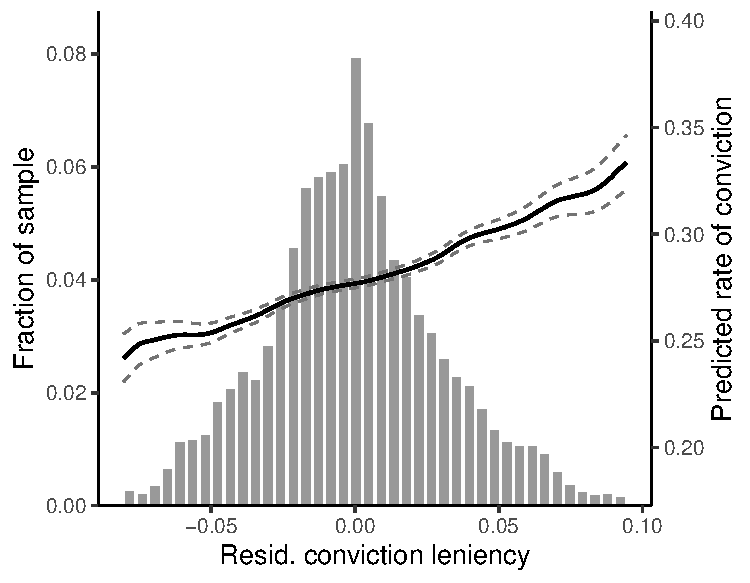
\includegraphics[width=\linewidth]{figures/first_stage_secondary_all.pdf}
\caption{All defendants, no score}
\end{subfigure}\hspace{0.04\textwidth}
\begin{subfigure}{0.42\textwidth}
\centering
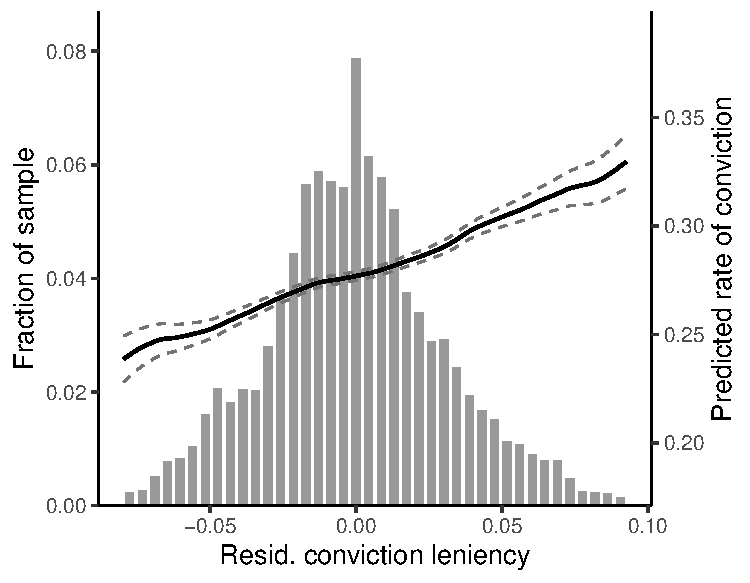
\includegraphics[width=\linewidth]{figures/first_stage_secondary_score_all.pdf}
\caption{All defendants, predicted score}
\end{subfigure}

\begin{subfigure}{0.42\textwidth}
\centering
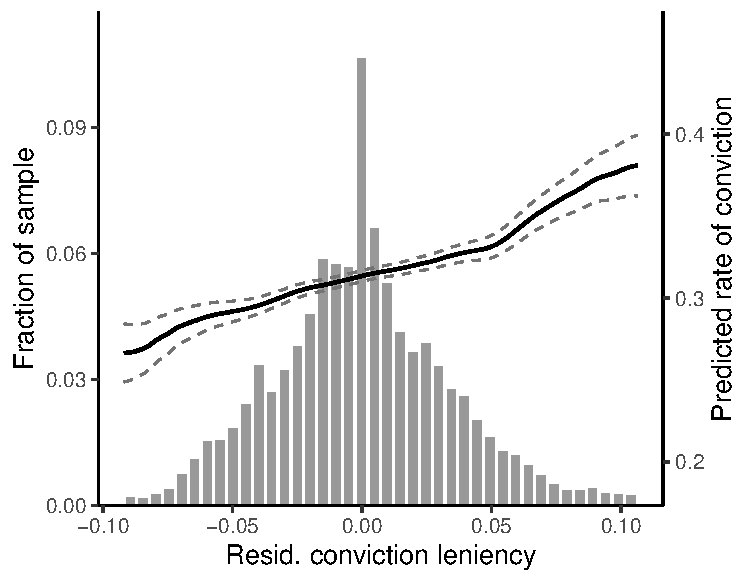
\includegraphics[width=\linewidth]{figures/first_stage_secondary_white.pdf}
\caption{White defendants, no score}
\end{subfigure}\hspace{0.04\textwidth}
\begin{subfigure}{0.42\textwidth}
\centering
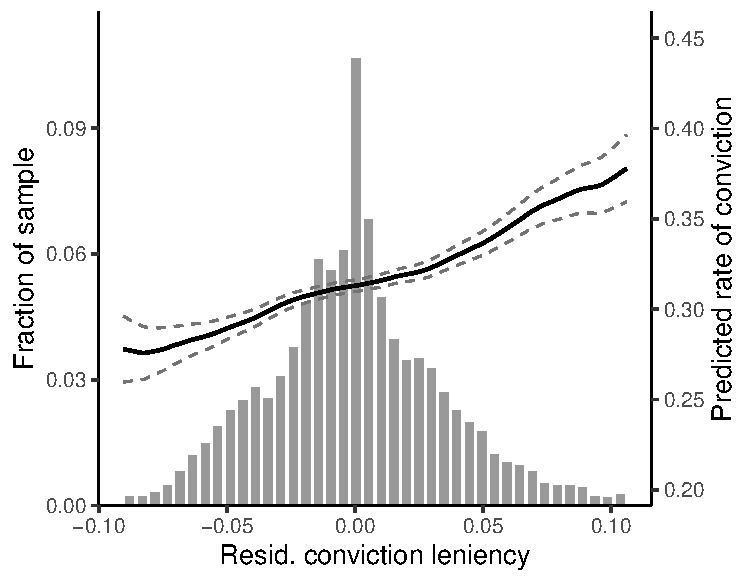
\includegraphics[width=\linewidth]{figures/first_stage_secondary_score_white.pdf}
\caption{White defendants, predicted score}
\end{subfigure}

\begin{subfigure}{0.42\textwidth}
\centering
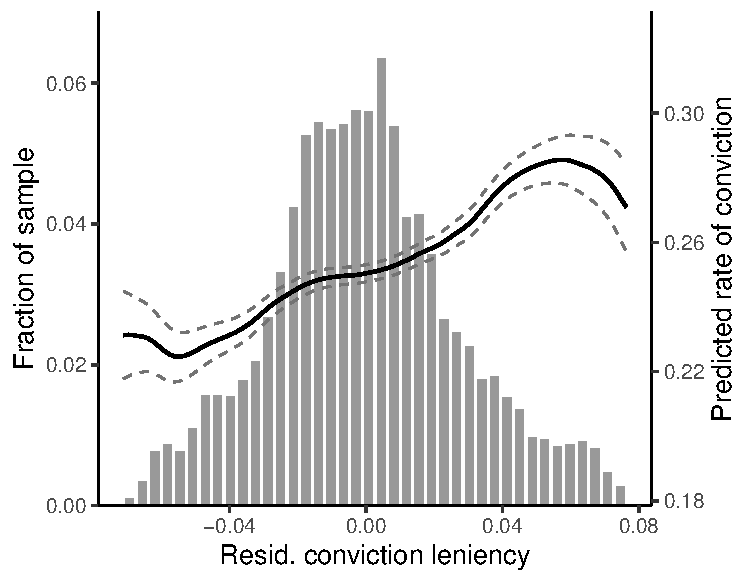
\includegraphics[width=\linewidth]{figures/first_stage_secondary_black.pdf}
\caption{Black defendants, no score}
\end{subfigure}\hspace{0.04\textwidth}
\begin{subfigure}{0.42\textwidth}
\centering
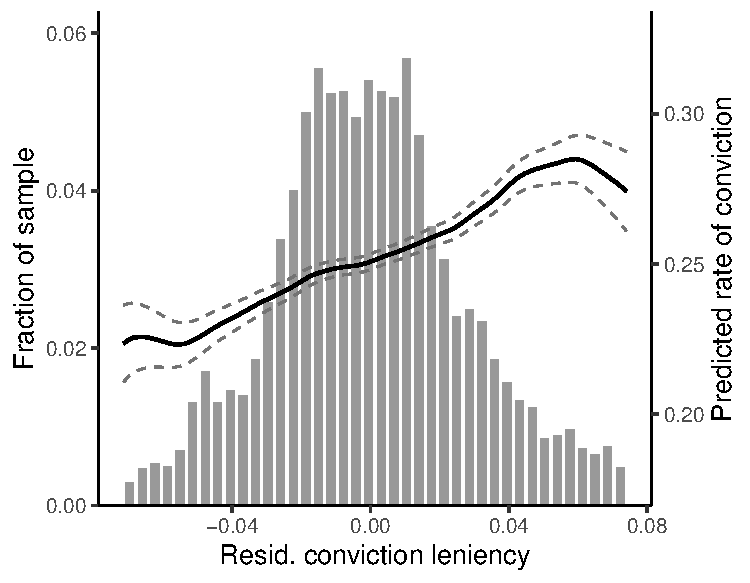
\includegraphics[width=\linewidth]{figures/first_stage_secondary_score_black.pdf}
\caption{Black defendants, predicted score}
\end{subfigure}
\caption{Distribution of conviction leniency and the first stage, secondary analysis}\label{fig:fs_secondary}
\tabnote{All cases. Histogram (left axis): conviction leniency net of the controls and fixed effects (not dismissal leniency), 1st--99th percentiles. Solid line (right axis): local linear regression (Epanechnikov kernel, bandwidth equal to the standard deviation of the instrument) of non-carceral conviction net of the same controls, plus its mean, on the residualized instrument; dashed lines: 95\% confidence interval, clustered by defendant. Left column: without a score control; right column: the instrument and treatment also residualized on the predicted-score indicators. Instruments built within the defendant's race. \allnote{} \racesamplenote}
\end{figure}

\begin{figure}[H]
\centering
\begin{subfigure}{0.42\textwidth}
\centering
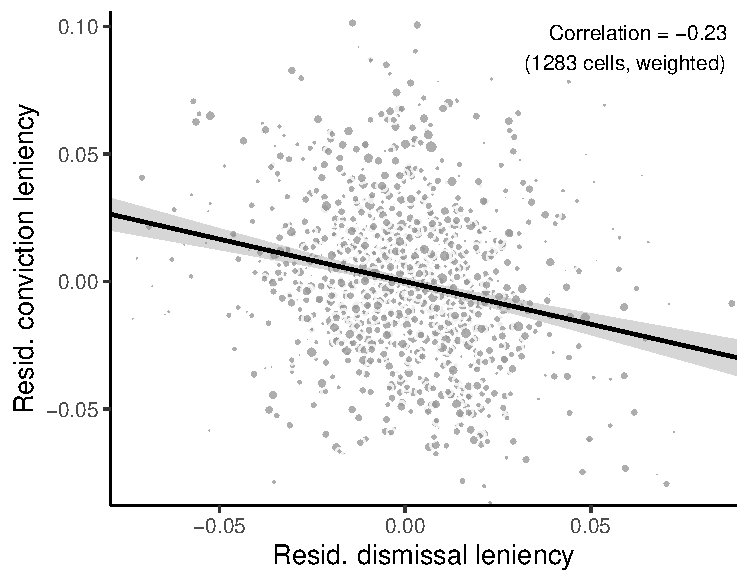
\includegraphics[width=\linewidth]{figures/leniency_scatter_secondary_all.pdf}
\caption{All defendants, no score}
\end{subfigure}\hspace{0.04\textwidth}
\begin{subfigure}{0.42\textwidth}
\centering
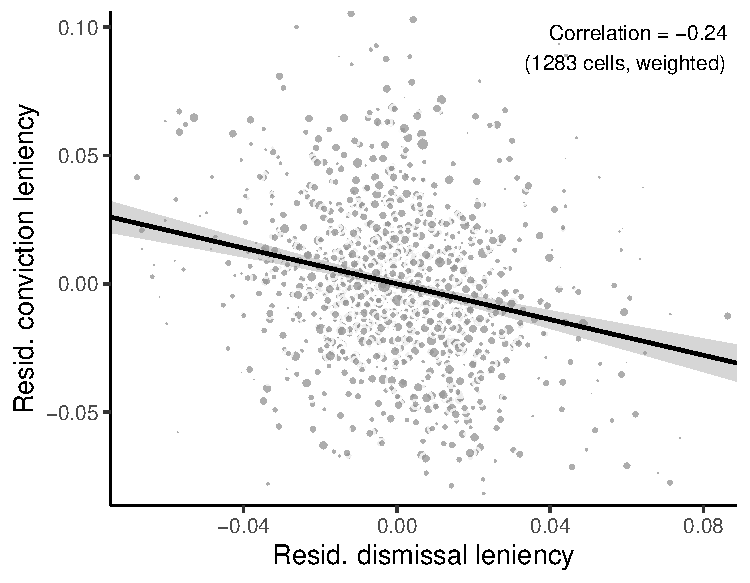
\includegraphics[width=\linewidth]{figures/leniency_scatter_secondary_score_all.pdf}
\caption{All defendants, predicted score}
\end{subfigure}

\begin{subfigure}{0.42\textwidth}
\centering
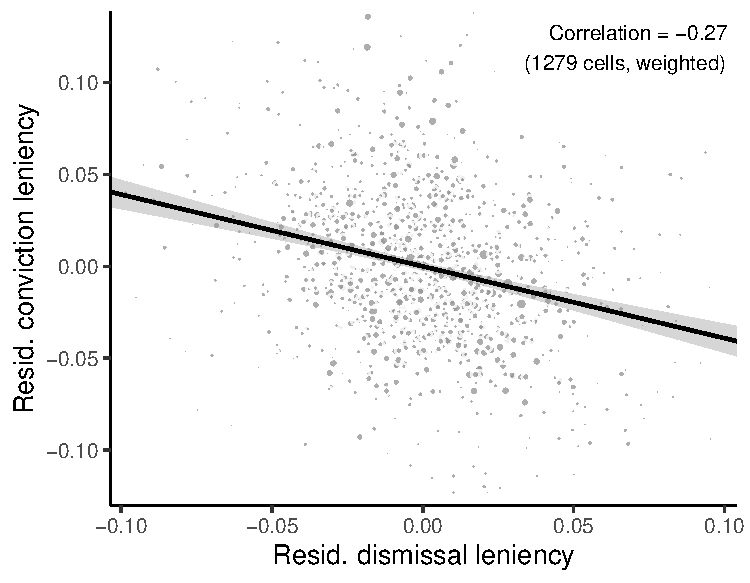
\includegraphics[width=\linewidth]{figures/leniency_scatter_secondary_white.pdf}
\caption{White defendants, no score}
\end{subfigure}\hspace{0.04\textwidth}
\begin{subfigure}{0.42\textwidth}
\centering
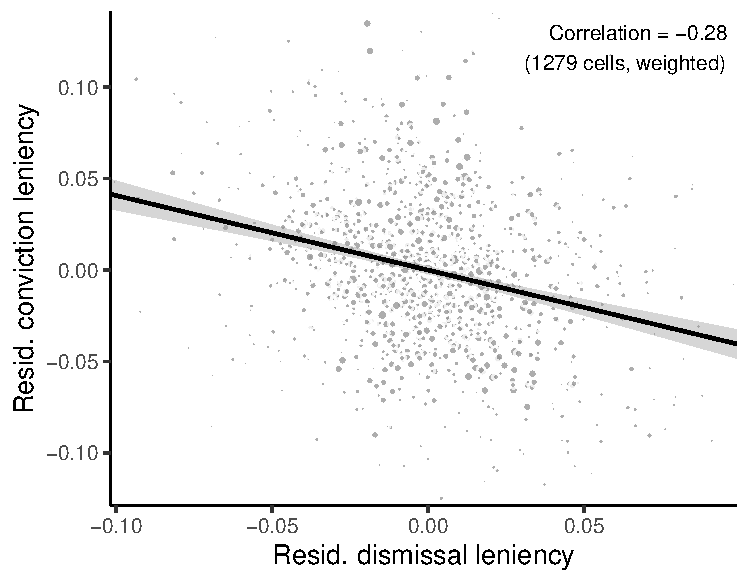
\includegraphics[width=\linewidth]{figures/leniency_scatter_secondary_score_white.pdf}
\caption{White defendants, predicted score}
\end{subfigure}

\begin{subfigure}{0.42\textwidth}
\centering
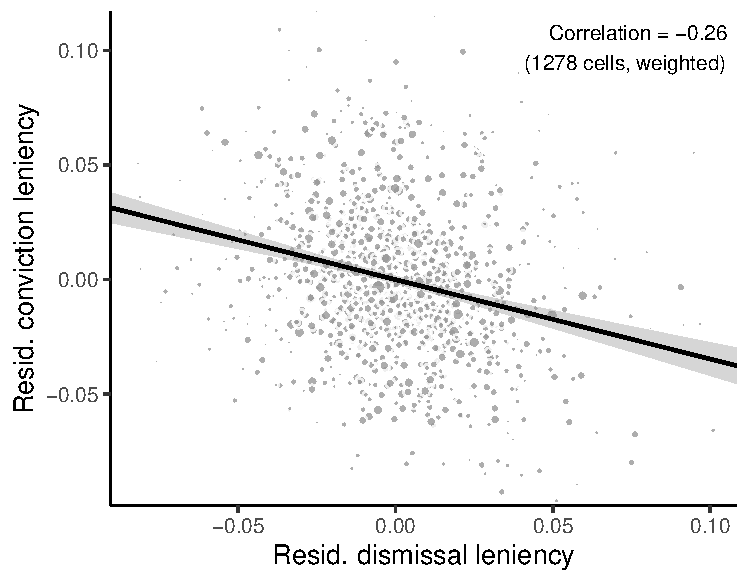
\includegraphics[width=\linewidth]{figures/leniency_scatter_secondary_black.pdf}
\caption{Black defendants, no score}
\end{subfigure}\hspace{0.04\textwidth}
\begin{subfigure}{0.42\textwidth}
\centering
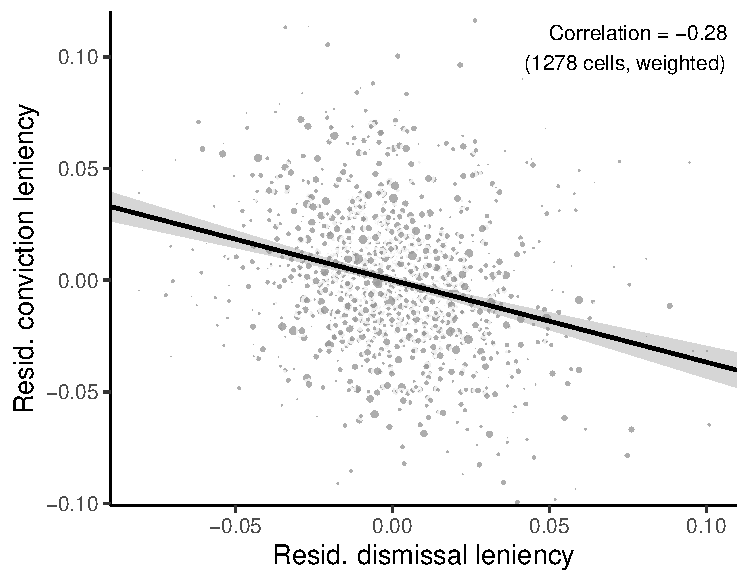
\includegraphics[width=\linewidth]{figures/leniency_scatter_secondary_score_black.pdf}
\caption{Black defendants, predicted score}
\end{subfigure}
\caption{Conviction leniency against dismissal leniency, secondary analysis}\label{fig:scatter_secondary}
\tabnote{Each point is a judge $\times$ year $\times$ court cell: conviction leniency against dismissal leniency, both built over all cases within the defendant's race, net of the controls and fixed effects and averaged over the cell's cases of the panel's defendants; point size proportional to the number of cases. \allnote{} Line: linear fit weighted by cases, with its 95\% confidence interval. Left column: without a score control; right column: with the predicted-score indicators. \racesamplenote}
\end{figure}

\begin{table}[H]
\centering
\caption{Balance: non-carceral conviction and conviction leniency, secondary analysis}\label{tab:balance_secondary}
\resizebox{\textwidth}{!}{% Secondary instruments. Balance: non-carceral conviction (Conviction) and the conviction instrument
% (loo_d1_jyr_race / loo_d1_jyr_pred_race; Leniency) regressed on the covariates, with fixed
% effects: court x year, court x calendar month, court x day of week. Columns 'Predicted score': the
% instruments (loo_d1_jyr_pred, loo_d0_jyr_pred; by race loo_d1_jyr_pred_race, loo_d0_jyr_pred_race)
% built, and the regressions estimated, also with one indicator per rounded value of the predicted
% sentencing score (05). All defendants: White and Black defendants, the fixed effects specific to
% each race. Any misdemeanor charge: in the case. Prior convictions between 31 days and 5 years before
% the case's first offense: felony, a convicted felony case in the full circuit-court record or a
% Sentencing Commission sentencing event of the defendant; misdemeanor only, a convicted misdemeanor
% circuit-court case and no felony conviction. Standard errors clustered by defendant; joint F-test of
% all covariates. White and Black defendants: only the cases of judges with at least 50 cases of White
% and 50 of Black defendants in the case's 3-year window.
\begin{tabular}{lcccccccccccc}
\toprule
 & \multicolumn{4}{c}{All} & \multicolumn{4}{c}{White} & \multicolumn{4}{c}{Black} \\
\cmidrule(lr){2-5}\cmidrule(lr){6-9}\cmidrule(lr){10-13}
 & \multicolumn{2}{c}{No score} & \multicolumn{2}{c}{Predicted score} & \multicolumn{2}{c}{No score} & \multicolumn{2}{c}{Predicted score} & \multicolumn{2}{c}{No score} & \multicolumn{2}{c}{Predicted score} \\
\cmidrule(lr){2-3}\cmidrule(lr){4-5}\cmidrule(lr){6-7}\cmidrule(lr){8-9}\cmidrule(lr){10-11}\cmidrule(lr){12-13}
 & Conviction & Leniency & Conviction & Leniency & Conviction & Leniency & Conviction & Leniency & Conviction & Leniency & Conviction & Leniency \\
 & (1) & (2) & (3) & (4) & (5) & (6) & (7) & (8) & (9) & (10) & (11) & (12) \\
\midrule
Female & $0.1065^{***}$ & $-0.0000$ & $0.0755^{***}$ & $-0.0000$ & $0.0813^{***}$ & $-0.0001$ & $0.0604^{***}$ & $-0.0001$ & $0.1270^{***}$ & $0.0001$ & $0.0896^{***}$ & $0.0001$ \\
 & (0.0023) & (0.0002) & (0.0023) & (0.0002) & (0.0034) & (0.0003) & (0.0033) & (0.0003) & (0.0033) & (0.0002) & (0.0032) & (0.0002) \\
Prior felony conviction (5 years) & $-0.1320^{***}$ & $-0.0002$ & $-0.0327^{***}$ & $-0.0003^{*}$ & $-0.1371^{***}$ & $-0.0003$ & $-0.0353^{***}$ & $-0.0005$ & $-0.1282^{***}$ & $-0.0001$ & $-0.0318^{***}$ & $-0.0002$ \\
 & (0.0019) & (0.0002) & (0.0021) & (0.0002) & (0.0031) & (0.0003) & (0.0037) & (0.0004) & (0.0023) & (0.0002) & (0.0025) & (0.0002) \\
Prior misdemeanor only conviction (5 years) & $-0.0566^{***}$ & $0.0003$ & $-0.0230^{***}$ & $0.0003$ & $-0.0592^{***}$ & $0.0007$ & $-0.0299^{***}$ & $0.0006$ & $-0.0532^{***}$ & $0.0001$ & $-0.0173^{***}$ & $0.0001$ \\
 & (0.0040) & (0.0003) & (0.0040) & (0.0003) & (0.0065) & (0.0006) & (0.0064) & (0.0006) & (0.0051) & (0.0004) & (0.0050) & (0.0004) \\
Offense: assault & $-0.1270^{***}$ & $-0.0005^{**}$ & $-0.0536^{***}$ & $-0.0006^{**}$ & $-0.1410^{***}$ & $-0.0004$ & $-0.0630^{***}$ & $-0.0006$ & $-0.1240^{***}$ & $-0.0006^{*}$ & $-0.0508^{***}$ & $-0.0006^{**}$ \\
 & (0.0028) & (0.0003) & (0.0029) & (0.0003) & (0.0051) & (0.0005) & (0.0053) & (0.0005) & (0.0034) & (0.0003) & (0.0035) & (0.0003) \\
Offense: burglary & $-0.0376^{***}$ & $-0.0001$ & $0.0188^{***}$ & $-0.0000$ & $-0.0466^{***}$ & $0.0004$ & $0.0139^{**}$ & $0.0005$ & $-0.0321^{***}$ & $-0.0004$ & $0.0202^{***}$ & $-0.0003$ \\
 & (0.0035) & (0.0003) & (0.0035) & (0.0003) & (0.0055) & (0.0005) & (0.0057) & (0.0005) & (0.0044) & (0.0003) & (0.0045) & (0.0003) \\
Offense: drugs & $-0.0084^{***}$ & $0.0003$ & $-0.0380^{***}$ & $0.0004^{*}$ & $0.0075^{*}$ & $-0.0002$ & $-0.0352^{***}$ & $-0.0002$ & $-0.0193^{***}$ & $0.0007^{***}$ & $-0.0389^{***}$ & $0.0007^{***}$ \\
 & (0.0025) & (0.0002) & (0.0026) & (0.0002) & (0.0043) & (0.0004) & (0.0044) & (0.0004) & (0.0031) & (0.0002) & (0.0032) & (0.0002) \\
Offense: fraud & $0.0393^{***}$ & $0.0002$ & $0.1053^{***}$ & $0.0002$ & $0.0307^{***}$ & $0.0001$ & $0.0970^{***}$ & $0.0003$ & $0.0434^{***}$ & $0.0003$ & $0.1072^{***}$ & $0.0002$ \\
 & (0.0033) & (0.0003) & (0.0035) & (0.0003) & (0.0051) & (0.0004) & (0.0053) & (0.0004) & (0.0045) & (0.0003) & (0.0046) & (0.0003) \\
Offense: kidnapping & $-0.0644^{***}$ & $-0.0011^{**}$ & $-0.0457^{***}$ & $-0.0011^{**}$ & $-0.0776^{***}$ & $-0.0003$ & $-0.0542^{***}$ & $-0.0004$ & $-0.0614^{***}$ & $-0.0014^{**}$ & $-0.0437^{***}$ & $-0.0014^{**}$ \\
 & (0.0051) & (0.0005) & (0.0050) & (0.0005) & (0.0102) & (0.0012) & (0.0100) & (0.0012) & (0.0058) & (0.0006) & (0.0057) & (0.0006) \\
Offense: larceny & $-0.0012$ & $0.0002$ & $-0.0704^{***}$ & $0.0003$ & $-0.0057$ & $0.0000$ & $-0.0686^{***}$ & $0.0000$ & $0.0006$ & $0.0004^{*}$ & $-0.0737^{***}$ & $0.0004$ \\
 & (0.0026) & (0.0002) & (0.0027) & (0.0002) & (0.0041) & (0.0003) & (0.0043) & (0.0004) & (0.0033) & (0.0002) & (0.0035) & (0.0003) \\
Offense: miscellaneous & $0.0056$ & $-0.0007^{*}$ & $0.0353^{***}$ & $-0.0006^{*}$ & $-0.0090$ & $-0.0005$ & $0.0230^{***}$ & $-0.0005$ & $0.0152^{***}$ & $-0.0008^{*}$ & $0.0416^{***}$ & $-0.0008^{*}$ \\
 & (0.0044) & (0.0003) & (0.0043) & (0.0003) & (0.0068) & (0.0006) & (0.0068) & (0.0006) & (0.0057) & (0.0004) & (0.0057) & (0.0004) \\
Offense: murder & $-0.1485^{***}$ & $-0.0005$ & $-0.1122^{***}$ & $-0.0005$ & $-0.2202^{***}$ & $0.0011$ & $-0.1650^{***}$ & $0.0010$ & $-0.1258^{***}$ & $-0.0009$ & $-0.0936^{***}$ & $-0.0010$ \\
 & (0.0049) & (0.0007) & (0.0047) & (0.0007) & (0.0104) & (0.0016) & (0.0102) & (0.0016) & (0.0055) & (0.0007) & (0.0053) & (0.0007) \\
Offense: robbery & $-0.0846^{***}$ & $0.0000$ & $-0.0381^{***}$ & $0.0000$ & $-0.1411^{***}$ & $-0.0002$ & $-0.0821^{***}$ & $-0.0003$ & $-0.0695^{***}$ & $0.0002$ & $-0.0238^{***}$ & $0.0002$ \\
 & (0.0036) & (0.0003) & (0.0036) & (0.0004) & (0.0076) & (0.0009) & (0.0076) & (0.0009) & (0.0041) & (0.0004) & (0.0041) & (0.0004) \\
Offense: sex assault & $-0.1590^{***}$ & $0.0000$ & $-0.0803^{***}$ & $-0.0002$ & $-0.1910^{***}$ & $0.0007$ & $-0.1052^{***}$ & $0.0003$ & $-0.1300^{***}$ & $-0.0008$ & $-0.0596^{***}$ & $-0.0009$ \\
 & (0.0053) & (0.0006) & (0.0053) & (0.0006) & (0.0074) & (0.0009) & (0.0075) & (0.0009) & (0.0075) & (0.0007) & (0.0074) & (0.0007) \\
Offense: sex offense & $-0.1092^{***}$ & $-0.0004$ & $-0.0606^{***}$ & $-0.0004$ & $-0.1227^{***}$ & $-0.0011$ & $-0.0713^{***}$ & $-0.0011$ & $-0.0906^{***}$ & $0.0011$ & $-0.0544^{***}$ & $0.0011$ \\
 & (0.0074) & (0.0007) & (0.0073) & (0.0007) & (0.0092) & (0.0009) & (0.0092) & (0.0010) & (0.0124) & (0.0012) & (0.0123) & (0.0012) \\
Offense: traffic & $-0.1650^{***}$ & $-0.0002$ & $-0.1059^{***}$ & $-0.0002$ & $-0.2084^{***}$ & $-0.0003$ & $-0.1589^{***}$ & $-0.0004$ & $-0.1279^{***}$ & $-0.0002$ & $-0.0604^{***}$ & $-0.0001$ \\
 & (0.0032) & (0.0003) & (0.0033) & (0.0003) & (0.0049) & (0.0005) & (0.0050) & (0.0005) & (0.0042) & (0.0004) & (0.0043) & (0.0004) \\
Offense: weapon & $-0.1153^{***}$ & $-0.0005^{*}$ & $-0.0395^{***}$ & $-0.0006^{**}$ & $-0.0939^{***}$ & $-0.0016^{**}$ & $-0.0086$ & $-0.0018^{**}$ & $-0.1182^{***}$ & $-0.0002$ & $-0.0451^{***}$ & $-0.0003$ \\
 & (0.0031) & (0.0003) & (0.0032) & (0.0003) & (0.0079) & (0.0007) & (0.0080) & (0.0007) & (0.0034) & (0.0003) & (0.0035) & (0.0003) \\
Any misdemeanor charge & $-0.0118^{***}$ & $0.0001$ & $-0.0146^{***}$ & $0.0001$ & $-0.0121^{***}$ & $0.0003$ & $-0.0151^{***}$ & $0.0003$ & $-0.0107^{***}$ & $-0.0001$ & $-0.0134^{***}$ & $-0.0000$ \\
 & (0.0028) & (0.0002) & (0.0028) & (0.0002) & (0.0043) & (0.0004) & (0.0043) & (0.0004) & (0.0037) & (0.0003) & (0.0036) & (0.0003) \\
\midrule
Joint F-statistic & 1,293.44 & 2.11 & 413.46 & 2.10 & 531.53 & 0.78 & 203.94 & 0.92 & 807.10 & 3.15 & 235.21 & 2.65 \\
Joint F-test p-value & 0.000 & 0.005 & 0.000 & 0.005 & 0.000 & 0.720 & 0.000 & 0.553 & 0.000 & 0.000 & 0.000 & 0.000 \\
Mean of dependent variable & 0.2779 & $-$0.0002 & 0.2779 & $-$0.0002 & 0.3136 & $-$0.0002 & 0.3136 & $-$0.0002 & 0.2522 & $-$0.0002 & 0.2522 & $-$0.0002 \\
Observations & 263,685 & 263,685 & 263,685 & 263,685 & 110,131 & 110,131 & 110,131 & 110,131 & 153,554 & 153,554 & 153,554 & 153,554 \\
Predicted-score control & No & No & Yes & Yes & No & No & Yes & Yes & No & No & Yes & Yes \\
\bottomrule
\multicolumn{13}{l}{\footnotesize $^{*}$ p $<$ 0.1, $^{**}$ p $<$ 0.05, $^{***}$ p $<$ 0.01} \\
\end{tabular}
}
\tabnote{All cases. For each group and specification: non-carceral conviction (first column) and conviction leniency (second column), each regressed on the covariates with court $\times$ year, court $\times$ calendar month and court $\times$ day-of-week fixed effects and, in the predicted-score columns, an indicator for each rounded value of the predicted score. \allnote{} Joint $F$-statistic and $p$-value: Wald test that all covariate coefficients are zero. Standard errors, in parentheses, clustered by defendant. \racesamplenote}
\end{table}

\begin{table}[H]
\centering
\caption{Split-sample monotonicity: first stages, secondary analysis}\label{tab:mono_secondary}
\resizebox{\textwidth}{!}{% Secondary instruments. Split-sample monotonicity: for each split, the conviction instrument is
% built from one group only and the first stage of non-carceral conviction on it is estimated on
% the other group, controlling for the dismissal instrument built from the same group; coefficient
% on the conviction instrument and (standard error). Controls and fixed effects as in the first
% stages, without the controls constant within the group; standard errors clustered by defendant.
% The conviction instrument is built from the cases of the defendant's race (as in the analysis),
% restricted to the group; the dismissal instrument from all cases of the race. All defendants (White
% and Black): the race split builds the instruments from one race's cases and estimates the first
% stage on the other race; the other splits build each race's instruments from that race's cases of
% the group and estimate the first stage on both races, every control and fixed effect specific to
% each race and one coefficient on each instrument, so the coefficient is a weighted average of the
% White and Black ones. Columns 'Predicted score': the instruments (loo_d1_jyr_pred, loo_d0_jyr_pred;
% by race loo_d1_jyr_pred_race, loo_d0_jyr_pred_race) built, and the regressions estimated, also with
% one indicator per rounded value of the predicted sentencing score (05). White and Black defendants:
% only the cases of judges with at least 50 cases of White and 50 of Black defendants in the case's
% 3-year window.
\begin{tabular}{lcccccc}
\toprule
 & \multicolumn{2}{c}{All} & \multicolumn{2}{c}{White} & \multicolumn{2}{c}{Black} \\
\cmidrule(lr){2-3}\cmidrule(lr){4-5}\cmidrule(lr){6-7}
Instrument built from $\rightarrow$ first stage on & No score & Predicted score & No score & Predicted score & No score & Predicted score \\
\midrule
\multicolumn{7}{l}{\textit{Race}} \\
White $\rightarrow$ Black & $0.392^{***}$ & $0.406^{***}$ &  &  &  &  \\
 & (0.027) & (0.026) &  &  &  &  \\
Black $\rightarrow$ White & $0.680^{***}$ & $0.732^{***}$ &  &  &  &  \\
 & (0.045) & (0.045) &  &  &  &  \\
\addlinespace
\multicolumn{7}{l}{\textit{Sex}} \\
Male $\rightarrow$ Female & $0.649^{***}$ & $0.654^{***}$ & $0.672^{***}$ & $0.671^{***}$ & $0.633^{***}$ & $0.646^{***}$ \\
 & (0.060) & (0.059) & (0.077) & (0.076) & (0.094) & (0.093) \\
Female $\rightarrow$ Male & $0.222^{***}$ & $0.221^{***}$ & $0.246^{***}$ & $0.243^{***}$ & $0.204^{***}$ & $0.205^{***}$ \\
 & (0.017) & (0.017) & (0.027) & (0.027) & (0.022) & (0.022) \\
\addlinespace
\multicolumn{7}{l}{\textit{Prior felony conviction (5 years)}} \\
No prior felony $\rightarrow$ Prior felony & $0.537^{***}$ & $0.579^{***}$ & $0.547^{***}$ & $0.583^{***}$ & $0.532^{***}$ & $0.579^{***}$ \\
 & (0.046) & (0.046) & (0.071) & (0.071) & (0.059) & (0.059) \\
Prior felony $\rightarrow$ No prior felony & $0.220^{***}$ & $0.227^{***}$ & $0.176^{***}$ & $0.186^{***}$ & $0.283^{***}$ & $0.286^{***}$ \\
 & (0.021) & (0.020) & (0.027) & (0.027) & (0.032) & (0.031) \\
\bottomrule
\multicolumn{7}{l}{\footnotesize $^{*}$ p $<$ 0.1, $^{**}$ p $<$ 0.05, $^{***}$ p $<$ 0.01} \\
\end{tabular}
}
\tabnote{Each coefficient: first stage of non-carceral conviction on conviction leniency built from the cases of one group only (``built from $\rightarrow$ first stage on''), estimated on the cases of the other group, controlling for dismissal leniency built from the same group; all cases, instruments built within the defendant's race, without and with the predicted-score indicators. All defendants: the race split builds the instruments from one race's cases and estimates the first stage on the other race; the other splits build each race's instruments from that race's cases of the group and estimate the first stage on both races, with the controls and fixed effects specific to each race and one coefficient on each instrument. \racesamplenote}
\end{table}

\begin{table}[H]
\centering
\caption{Who decides the defendants' revocation proceedings and new felony cases, secondary analysis}\label{tab:rev_judges_sec}
{\small\setlength{\tabcolsep}{4pt}\renewcommand{\arraystretch}{0.9}\resizebox{\textwidth}{!}{% Secondary analysis. White and Black defendants of the race samples, cases first disposed in or
% before 2016: their felony revocation proceedings (charges of a case filed on one date) filed within
% 3 years after the focal disposition, by the revocation measure that counts them and the case they
% are filed under, and their new felony cases (judge-IV cases) charged within 3 years. N: proceedings
% (cases) with judge information on their pleadings. Focal judge: share decided by the focal case's
% judge. At random: share expected if the deciding judge were drawn in proportion to the judges'
% caseloads in the court and year (all felony revocation proceedings, or all judge-IV cases), zero in
% another court.
\begin{tabular}{lccc}
\toprule
 & N & Focal judge (\%) & At random (\%) \\
\midrule
\multicolumn{4}{l}{\textit{Counted in the primary revocation measure (other sentences)}} \\
\quad Revocation proceedings: later sentences & 9,452 & 18 & 12 \\
\quad Revocation proceedings: earlier sentences, after a new case & 6,083 & 16 & 12 \\
\quad Revocation proceedings: revocation-only case nos., after a new case & 2,014 & 23 & 16 \\
\quad Revocation proceedings: all of the primary measure & 17,549 & 18 & 13 \\
\addlinespace
\multicolumn{4}{l}{\textit{Counted in the secondary revocation measure (focal sentences)}} \\
\quad Revocation proceedings: filed under the focal case & 47,295 & 60 & 20 \\
\quad Revocation proceedings: other cases sentenced at the focal hearing & 6,573 & 54 & 22 \\
\quad Revocation proceedings: all of the secondary measure & 53,868 & 60 & 21 \\
\addlinespace
\multicolumn{4}{l}{\textit{Counted in neither revocation measure}} \\
\quad Revocation proceedings: earlier or unidentified, no new case & 24,370 & 20 & 14 \\
\addlinespace
\multicolumn{4}{l}{\textit{Not revocation proceedings}} \\
\quad New felony cases (not revocation proceedings) & 53,462 & 14 & 12 \\
\bottomrule
\end{tabular}
}}
\tabnote{White and Black defendants of the secondary race samples, cases first disposed in or before 2016: their felony revocation proceedings filed within three years after the focal disposition, grouped by the measure that counts them and the case they are filed under, and their new felony cases (judge-IV cases) charged within three years. N: proceedings (cases) with judge information on their pleadings. Focal judge: the share decided by the focal case's judge. At random: the share expected if the deciding judge were drawn in proportion to the judges' caseloads in the court and year, zero in another court. \racesamplenote}
\end{table}

\begin{figure}[H]
\centering
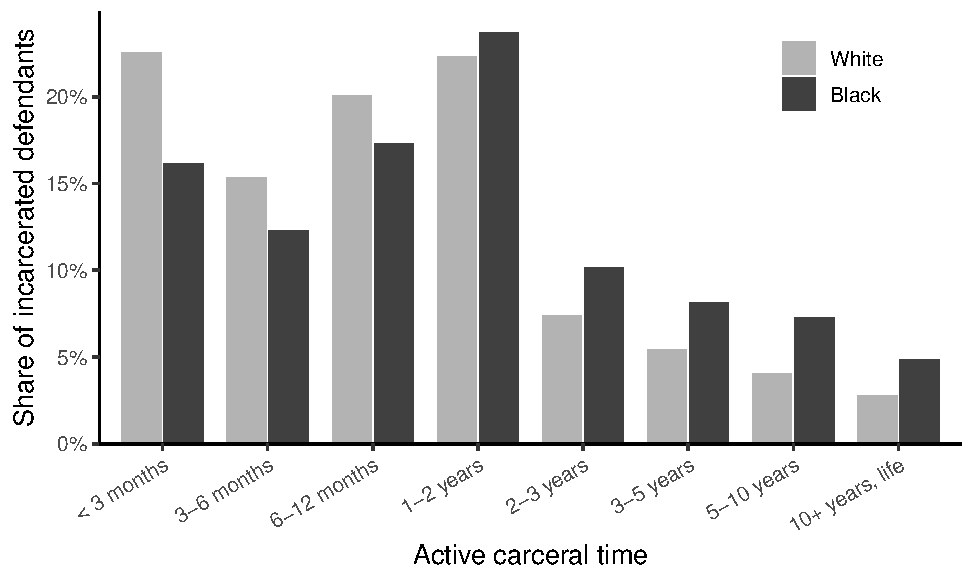
\includegraphics[width=0.8\textwidth]{figures/sentence_length_secondary.pdf}
\caption{Active carceral time of incarcerated defendants, by race, secondary analysis}\label{fig:sentence_length_sec}
\tabnote{Incarcerated defendants (carceral sentence in the focal case) of the secondary race samples, cases first disposed in or before 2016 (50,667 White and 79,144 Black defendants): share of each race's incarcerated defendants by active carceral time, the jail and penitentiary time net of the suspended part, with the case's sentences consecutive unless the court made them concurrent; life and death sentences in the last bin. Bins include their lower bound. \racesamplenote}
\end{figure}

\begin{table}[H]
\centering
\caption{Recidivism of incarcerated defendants from the disposition, by race, secondary analysis}\label{tab:recid_inc_sec}
\resizebox{\textwidth}{!}{% Secondary instruments' sample. Share of incarcerated defendants (d2 = 1, analysis sample) with any
% new felony CC case charged / convicted / incarcerated, any revocation proceeding / revocation of
% the person's other felony sentences, or of the focal felony sentences (04), within 1, 2 and 3 years
% after the case's first disposition; all outcomes on the cases first disposed in or before 2016 (full
% follow-up for 3 years in the circuit-court record, which ends in 2019). Stars: test that the share
% is zero; standard errors, in parentheses, clustered by person. White and Black defendants: only
% the cases of judges with at least 50 cases of White and 50 of Black defendants in the case's 3-year
% window.
\begin{tabular}{lcccccc}
\toprule
 & \multicolumn{2}{c}{1 year} & \multicolumn{2}{c}{2 years} & \multicolumn{2}{c}{3 years} \\
\cmidrule(lr){2-3}\cmidrule(lr){4-5}\cmidrule(lr){6-7}
 & White & Black & White & Black & White & Black \\
\midrule
\multicolumn{7}{l}{\textit{New felony CC case}} \\
Charged & $0.064^{***}$ & $0.067^{***}$ & $0.129^{***}$ & $0.140^{***}$ & $0.183^{***}$ & $0.203^{***}$ \\
 & (0.001) & (0.001) & (0.002) & (0.001) & (0.002) & (0.002) \\
Convicted & $0.059^{***}$ & $0.059^{***}$ & $0.119^{***}$ & $0.125^{***}$ & $0.170^{***}$ & $0.182^{***}$ \\
 & (0.001) & (0.001) & (0.002) & (0.001) & (0.002) & (0.002) \\
Incarcerated & $0.048^{***}$ & $0.051^{***}$ & $0.097^{***}$ & $0.108^{***}$ & $0.140^{***}$ & $0.158^{***}$ \\
 & (0.001) & (0.001) & (0.001) & (0.001) & (0.002) & (0.001) \\
\addlinespace
\multicolumn{7}{l}{\textit{Revocation of the person's other sentences}} \\
Proceeding & $0.013^{***}$ & $0.011^{***}$ & $0.043^{***}$ & $0.036^{***}$ & $0.077^{***}$ & $0.066^{***}$ \\
 & (0.001) & (0.000) & (0.001) & (0.001) & (0.001) & (0.001) \\
Revoked & $0.012^{***}$ & $0.009^{***}$ & $0.040^{***}$ & $0.032^{***}$ & $0.071^{***}$ & $0.060^{***}$ \\
 & (0.001) & (0.000) & (0.001) & (0.001) & (0.001) & (0.001) \\
\addlinespace
\multicolumn{7}{l}{\textit{Revocation of the focal sentences}} \\
Proceeding & $0.083^{***}$ & $0.077^{***}$ & $0.178^{***}$ & $0.167^{***}$ & $0.241^{***}$ & $0.234^{***}$ \\
 & (0.001) & (0.001) & (0.002) & (0.001) & (0.002) & (0.002) \\
Revoked & $0.070^{***}$ & $0.066^{***}$ & $0.155^{***}$ & $0.147^{***}$ & $0.210^{***}$ & $0.207^{***}$ \\
 & (0.001) & (0.001) & (0.002) & (0.001) & (0.002) & (0.002) \\
\midrule
Incarcerated defendants (cases) & 50,667 & 79,144 & 50,667 & 79,144 & 50,667 & 79,144 \\
\bottomrule
\multicolumn{7}{l}{\footnotesize $^{*}$ p $<$ 0.1, $^{**}$ p $<$ 0.05, $^{***}$ p $<$ 0.01} \\
\end{tabular}
}
\tabnote{Share of incarcerated defendants (carceral sentence in the focal case; all cases) with the outcome within 1, 2 or 3 years after the focal case's first disposition, on the cases first disposed in or before 2016. Revocations: the primary measure (the person's other sentences) and the secondary one (the focal sentences). Stars: test that the share is zero; standard errors, in parentheses, clustered by person. \racesamplenote}
\end{table}

\begin{table}[H]
\centering
\caption{Recidivism of incarcerated defendants from release, by race, secondary analysis}\label{tab:recid_inc_sec_rel}
\resizebox{\textwidth}{!}{% Secondary instruments' sample. Share of incarcerated defendants (d2 = 1, analysis sample) with any
% new felony CC case charged / convicted / incarcerated, any revocation proceeding / revocation of
% the person's other felony sentences, or of the focal felony sentences (04), within 1, 2 and 3 years
% after release from the focal sentence (first disposition plus 0.9 x active carceral time, at most
% 4 years); all outcomes on the cases first disposed in or before 2012 (full follow-up for 3 years in
% the circuit-court record, which ends in 2019). Stars: test that the share is zero; standard errors,
% in parentheses, clustered by person. White and Black defendants: only the cases of judges with at
% least 50 cases of White and 50 of Black defendants in the case's 3-year window.
\begin{tabular}{lcccccc}
\toprule
 & \multicolumn{2}{c}{1 year} & \multicolumn{2}{c}{2 years} & \multicolumn{2}{c}{3 years} \\
\cmidrule(lr){2-3}\cmidrule(lr){4-5}\cmidrule(lr){6-7}
 & White & Black & White & Black & White & Black \\
\midrule
\multicolumn{7}{l}{\textit{New felony CC case}} \\
Charged & $0.086^{***}$ & $0.102^{***}$ & $0.152^{***}$ & $0.182^{***}$ & $0.204^{***}$ & $0.247^{***}$ \\
 & (0.002) & (0.001) & (0.002) & (0.002) & (0.002) & (0.002) \\
Convicted & $0.078^{***}$ & $0.091^{***}$ & $0.140^{***}$ & $0.163^{***}$ & $0.190^{***}$ & $0.223^{***}$ \\
 & (0.002) & (0.001) & (0.002) & (0.002) & (0.002) & (0.002) \\
Incarcerated & $0.064^{***}$ & $0.077^{***}$ & $0.114^{***}$ & $0.141^{***}$ & $0.158^{***}$ & $0.193^{***}$ \\
 & (0.001) & (0.001) & (0.002) & (0.002) & (0.002) & (0.002) \\
\addlinespace
\multicolumn{7}{l}{\textit{Revocation of the person's other sentences}} \\
Proceeding & $0.024^{***}$ & $0.024^{***}$ & $0.060^{***}$ & $0.058^{***}$ & $0.094^{***}$ & $0.095^{***}$ \\
 & (0.001) & (0.001) & (0.001) & (0.001) & (0.002) & (0.001) \\
Revoked & $0.022^{***}$ & $0.021^{***}$ & $0.056^{***}$ & $0.052^{***}$ & $0.088^{***}$ & $0.087^{***}$ \\
 & (0.001) & (0.001) & (0.001) & (0.001) & (0.002) & (0.001) \\
\addlinespace
\multicolumn{7}{l}{\textit{Revocation of the focal sentences}} \\
Proceeding & $0.125^{***}$ & $0.132^{***}$ & $0.213^{***}$ & $0.224^{***}$ & $0.262^{***}$ & $0.279^{***}$ \\
 & (0.002) & (0.001) & (0.002) & (0.002) & (0.002) & (0.002) \\
Revoked & $0.109^{***}$ & $0.117^{***}$ & $0.187^{***}$ & $0.201^{***}$ & $0.231^{***}$ & $0.250^{***}$ \\
 & (0.002) & (0.001) & (0.002) & (0.002) & (0.002) & (0.002) \\
\midrule
Incarcerated defendants (cases) & 36,080 & 58,721 & 36,080 & 58,721 & 36,080 & 58,721 \\
\bottomrule
\multicolumn{7}{l}{\footnotesize $^{*}$ p $<$ 0.1, $^{**}$ p $<$ 0.05, $^{***}$ p $<$ 0.01} \\
\end{tabular}
}
\tabnote{As in Table~\ref{tab:recid_inc_sec}, with the outcomes within 1, 2 or 3 years after release from the focal sentence (the first disposition plus 90\% of the active carceral time, at most four years), on the cases first disposed in or before 2012.}
\end{table}

\subsection{Cross-validation with the ``Revolving Door'' paper}\label{sec:crossval}

\paragraph{Summary.} The Revolving Door paper (Humphries, Ouss, Stavreva, Stevenson and van Dijk 2025) estimates judge-IV effects of conviction and incarceration on future charges from the same circuit-court records; its Table E.7 reports them for Black and non-Black defendants. We reproduce Table E.7 exactly, and the paper's specification on our own sample gives estimates within about 0.06 of it. Our racial difference comes from building the instruments within race: with leniency measured over all defendants, the Black estimates fall and the White ones rise, reaching the paper's similar estimates for both groups once the instruments are also unresidualized, as the paper's are.

\paragraph{The steps.} Tables~\ref{tab:cv_conv} and~\ref{tab:cv_incar} move from our estimates of the effect on any future felony charge (year 1, years 2--4, 5--7 and 1--7 after sentencing) to Table E.7 as the paper's replication package produces it (data \texttt{final\_judge\_iv\_data.dta}; code \texttt{judge\_iv\_analysis\_\allowbreak convict\_and\_\allowbreak incar\_\allowbreak multinomial.do}), changing one element per row. All rows use the cases disposed by 2012 and the paper's two-instrument specification: non-carceral conviction (the paper's ``conviction'') is instrumented by conviction leniency controlling for incarceration leniency, so that the instrument shifts cases between non-carceral conviction and dismissal (our analyses control for dismissal leniency instead), and incarceration is instrumented by incarceration leniency controlling for dismissal leniency, so that it shifts cases between incarceration and non-carceral conviction. Rows (1)--(2) are from our secondary analysis, rows (3)--(7) apply the paper's specification to our sample, and rows (8)--(11) substitute the paper's data:
\begin{enumerate}
  \item[(1)] \emph{Our estimates}: the secondary analysis's race-specific residualized leave-out instruments (without the score control), controls, fixed effects and clustering, on judges with at least 50 cases of each race.
  \item[(2)] \emph{All judges}.
  \item[(3)] \emph{Same prior conviction controls}: the paper's felony flag (Sentencing Commission events only, 31 days to five years before the case) instead of ours (circuit-court or Sentencing Commission records), and no misdemeanor-only flag; the other controls already match.
  \item[(4)] \emph{Day-of-week FE} instead of court $\times$ day-of-week fixed effects.
  \item[(5)] \emph{Clustered by judge $\times$ year only}: the paper clusters by judge $\times$ year $\times$ court, and each judge-year sits in one court here (as in Stata's \texttt{ivregress}, no small-sample correction).
  \item[(6)] \emph{Pooled instruments}: built over all defendants rather than within race (still residualized).
  \item[(7)] \emph{Unresidualized instruments}: leave-out means of the raw decisions, with the controls and fixed effects only in the 2SLS. This row is the paper's specification on our sample: its instruments are raw leave-out means (\texttt{make\_\allowbreak data\_\allowbreak judge\_\allowbreak iv\_\allowbreak clean.do}, line 171, calls \texttt{gen\_loo\_\allowbreak instruments} with \texttt{window(3yr)} and \texttt{loo\_excl\_\allowbreak person} but not \texttt{residualized}).
  \item[(8)] \emph{Paper's cases}: our cases matched one-to-one to the paper's (99.7\% of them), with our variables.
  \item[(9)] \emph{Paper's outcome, treatment and instruments}: its future-charge indicator (any felony charge with an offense date in the window, excluding revocations and technical hearings), its treatment, and its instruments, built from its own data.
  \item[(10)] \emph{Paper's race indicator}: Black from the case's own charges (ours is the defendant's modal race), so the comparison group becomes non-Black defendants.
  \item[(11)] \emph{Paper's controls, FE, clusters and misc.}: the paper's own file, which adds its 901 unmatched cases (0.3\%) and its values of the controls, fixed-effect cells, clusters and years, and keeps a case the replication code counts twice (Appendix~\ref{sec:crossval_details}). This row reproduces Table E.7 exactly: coefficients, standard errors and observations.
\end{enumerate}
The two samples overlap almost completely: 276,164 cases match one-to-one (97.1\% of ours and 99.7\% of the paper's) and agree on the treatment for 99.4\% (Appendix~\ref{sec:crossval_details}).

\paragraph{Conviction.} Our estimates (Table~\ref{tab:cv_conv}, row 1) show effects of non-carceral conviction on future charges for Black defendants (0.18 in year 1 and 0.33 over years 1--7, both significant at 5\%) but not White defendants (0.08 and $-0.01$), whereas the paper finds similar effects for both (0.10 and 0.24 for each). The paper's controls, fixed effects and clustering (rows 3--5) move the years 1--7 estimates to 0.32 (Black) and 0.17 (White). Pooling the instruments (row 6) is the largest change: the Black estimate falls to 0.17 and the White one rises to 0.28 (year 1: 0.09 and 0.13). Leaving them unresidualized (row 7), which completes the paper's specification on our sample, brings both to 0.18 (year 1: 0.11 for Black and 0.08 for White defendants); the White estimate moves by about one standard error, the sampling variation that the case mix of the judges' other cases adds to an unresidualized instrument (main report, Section~6.2). The paper's data then move the estimates by at most about 0.09 per step: its cases (row 8) raise the Black estimate to 0.23, its outcome, treatment and instruments (row 9) the White one to 0.27, and its race indicator and remaining variables (rows 10--11) give 0.24 for both groups (significant at 5\% for non-Black and 10\% for Black defendants) and 0.10 for both in year 1.

\paragraph{Incarceration.} Our estimates (Table~\ref{tab:cv_incar}, row 1) show incarceration lowering future charges of Black defendants ($-0.21$ in year 1 and $-0.24$ over years 1--7, both significant) but not of White defendants (0.02 and 0.09); the paper finds $-0.13$ and $-0.12$ (the latter insignificant) for Black and $-0.05$ and $-0.02$ for non-Black defendants. Pooling the instruments (row 6) again accounts for most of the gap (Black: $-0.14$ and $-0.13$; White: $-0.06$ and $-0.04$), leaving them unresidualized (row 7) changes little (Black: $-0.15$ and $-0.13$; White: $-0.05$ and 0.00), and the paper's data (rows 8--11) move the estimates by at most about 0.03 per step.

\paragraph{Outcome.} Our outcome (rows 1--8), any new felony case charged in the window and dated by its first offense, has means of 0.303 (White) and 0.360 (Black) over years 1--7 and 0.071 and 0.080 in year 1 (all judges, cases disposed by 2012). The paper's (rows 9--11) has means of 0.291 (non-Black) and 0.359 (Black), and 0.069 and 0.081. The two agree for 99.4--99.7\% of matched cases.

\begin{table}[H]
\centering
\caption{From our estimates to Table E.7 of the Revolving Door paper: non-carceral conviction and future felony charges}\label{tab:cv_conv}
{\renewcommand{\arraystretch}{0.9}\resizebox{\textwidth}{!}{% Non-carceral conviction (2SLS) on any future felony charge in year 1, years 2-4, years 5-7 and
% years 1-7 after the case's first disposition, instrumented by conviction leniency, controlling for
% incarceration leniency: from our estimates (1) to Table E.7 of the Revolving Door paper (11), as its
% replication package makes it, each row changing one element of the row above; coefficient, (standard
% error), {observations}. (1): instruments built within the defendant's race; controls: offense type,
% any misdemeanor charge, prior felony conviction (circuit-court record or Sentencing Commission)
% and prior misdemeanor-only conviction between 31 days and 5 years before, female; fixed effects:
% court x year, court x calendar month, court x day of week; standard errors clustered by defendant;
% only the cases of judges with at least 50 cases of White and 50 of Black defendants in the case's
% 3-year window, as the analysis with instruments by race; (2) all judges. All rows on the cases first
% disposed in or before 2012 (full follow-up for every window). Paper's cases: ours matched one-to-one
% to the paper's (hashed case ids -> original case groups -> their charges -> our cases); (11): the
% paper's own data, which also adds its cases not matched to ours, its controls, FE cells, clusters
% and years, and each race group's 6th case counted twice, as the replication code does.
\begin{tabular}{lcccccccc}
\toprule
 & \multicolumn{4}{c}{White (non-Black from (10))} & \multicolumn{4}{c}{Black} \\
\cmidrule(lr){2-5}\cmidrule(lr){6-9}
 & Year 1 & Years 2--4 & Years 5--7 & Years 1--7 & Year 1 & Years 2--4 & Years 5--7 & Years 1--7 \\
\midrule
(1) Our estimates & $0.078$ & $-0.011$ & $-0.043$ & $-0.008$ & $0.176^{**}$ & $0.090$ & $0.158$ & $0.326^{**}$ \\
 & (0.085) & (0.125) & (0.118) & (0.151) & (0.087) & (0.129) & (0.123) & (0.157) \\
 & \{71,455\} & \{71,455\} & \{71,455\} & \{71,455\} & \{103,472\} & \{103,472\} & \{103,472\} & \{103,472\} \\
(2) All judges & $0.099$ & $0.063$ & $-0.041$ & $0.097$ & $0.159^{*}$ & $0.139$ & $0.163$ & $0.372^{**}$ \\
 & (0.079) & (0.115) & (0.110) & (0.139) & (0.087) & (0.131) & (0.124) & (0.160) \\
 & \{77,022\} & \{77,022\} & \{77,022\} & \{77,022\} & \{107,027\} & \{107,027\} & \{107,027\} & \{107,027\} \\
(3) Same prior conviction controls & $0.105$ & $0.084$ & $-0.024$ & $0.132$ & $0.157^{*}$ & $0.130$ & $0.154$ & $0.356^{**}$ \\
 & (0.081) & (0.118) & (0.112) & (0.143) & (0.086) & (0.130) & (0.123) & (0.159) \\
 & \{77,022\} & \{77,022\} & \{77,022\} & \{77,022\} & \{107,027\} & \{107,027\} & \{107,027\} & \{107,027\} \\
(4) Day-of-week FE & $0.113$ & $0.118$ & $-0.013$ & $0.174$ & $0.141^{*}$ & $0.118$ & $0.121$ & $0.315^{**}$ \\
 & (0.082) & (0.120) & (0.114) & (0.146) & (0.083) & (0.126) & (0.118) & (0.152) \\
 & \{77,022\} & \{77,022\} & \{77,022\} & \{77,022\} & \{107,027\} & \{107,027\} & \{107,027\} & \{107,027\} \\
(5) Clustered by judge $\times$ year only & $0.113$ & $0.118$ & $-0.013$ & $0.174$ & $0.141^{*}$ & $0.118$ & $0.121$ & $0.315^{*}$ \\
 & (0.071) & (0.111) & (0.109) & (0.136) & (0.078) & (0.128) & (0.122) & (0.164) \\
 & \{77,022\} & \{77,022\} & \{77,022\} & \{77,022\} & \{107,027\} & \{107,027\} & \{107,027\} & \{107,027\} \\
(6) Pooled instruments & $0.129^{**}$ & $0.176^{*}$ & $0.035$ & $0.280^{**}$ & $0.091$ & $0.025$ & $0.088$ & $0.165$ \\
 & (0.062) & (0.096) & (0.094) & (0.114) & (0.060) & (0.095) & (0.092) & (0.121) \\
 & \{77,022\} & \{77,022\} & \{77,022\} & \{77,022\} & \{107,027\} & \{107,027\} & \{107,027\} & \{107,027\} \\
(7) Unresidualized instruments & $0.080$ & $0.120$ & $0.011$ & $0.179$ & $0.108^{*}$ & $0.021$ & $0.112$ & $0.182$ \\
 & (0.061) & (0.093) & (0.091) & (0.111) & (0.063) & (0.098) & (0.094) & (0.126) \\
 & \{77,022\} & \{77,022\} & \{77,022\} & \{77,022\} & \{107,027\} & \{107,027\} & \{107,027\} & \{107,027\} \\
(8) Paper's cases & $0.084$ & $0.126$ & $-0.003$ & $0.182$ & $0.126^{*}$ & $0.024$ & $0.126$ & $0.225^{*}$ \\
 & (0.061) & (0.095) & (0.092) & (0.114) & (0.068) & (0.107) & (0.101) & (0.137) \\
 & \{74,819\} & \{74,819\} & \{74,819\} & \{74,819\} & \{103,950\} & \{103,950\} & \{103,950\} & \{103,950\} \\
(9) Paper's outcome, treatment and instruments & $0.119^{*}$ & $0.126$ & $0.050$ & $0.268^{**}$ & $0.092$ & $0.065$ & $0.101$ & $0.217$ \\
 & (0.066) & (0.098) & (0.101) & (0.124) & (0.068) & (0.114) & (0.106) & (0.142) \\
 & \{74,819\} & \{74,819\} & \{74,819\} & \{74,819\} & \{103,950\} & \{103,950\} & \{103,950\} & \{103,950\} \\
(10) Paper's race indicator & $0.104^{*}$ & $0.106$ & $0.038$ & $0.230^{**}$ & $0.097$ & $0.076$ & $0.108$ & $0.237$ \\
 & (0.062) & (0.089) & (0.093) & (0.113) & (0.068) & (0.114) & (0.107) & (0.145) \\
 & \{78,941\} & \{78,941\} & \{78,941\} & \{78,941\} & \{103,780\} & \{103,780\} & \{103,780\} & \{103,780\} \\
(11) Paper's controls, FE, clusters and misc. & $0.101$ & $0.114$ & $0.041$ & $0.237^{**}$ & $0.100$ & $0.076$ & $0.116$ & $0.244^{*}$ \\
 & (0.063) & (0.090) & (0.094) & (0.114) & (0.069) & (0.117) & (0.110) & (0.148) \\
 & \{79,158\} & \{79,158\} & \{79,158\} & \{79,158\} & \{104,225\} & \{104,225\} & \{104,225\} & \{104,225\} \\
\bottomrule
\multicolumn{9}{l}{\footnotesize $^{*}$ p $<$ 0.1, $^{**}$ p $<$ 0.05, $^{***}$ p $<$ 0.01} \\
\end{tabular}
}}
\tabnote{2SLS of any future felony charge in year 1, years 2--4, years 5--7 and years 1--7 after the case's first disposition on non-carceral conviction, instrumented by conviction leniency and controlling for incarceration leniency; coefficient, standard error in parentheses, and observations in braces. Each row changes one element of the row above (see the text); all rows on the cases first disposed by 2012. (1) our estimates, with the residualized instruments built within the defendant's race, on the cases of judges with at least 50 cases of each race; (2) all judges; (7) the paper's specification on our own analysis sample; (8)--(11) the paper's data, in turn; (11) Table E.7, Panel A, of the Revolving Door paper as its replication package produces it, exactly, including its duplicated 6th case of each race group (Appendix~\ref{sec:crossval_details}). From row (10) on, the first group is non-Black rather than White defendants.}
\end{table}

\begin{table}[H]
\centering
\caption{From our estimates to Table E.7 of the Revolving Door paper: incarceration and future felony charges}\label{tab:cv_incar}
{\renewcommand{\arraystretch}{0.9}\resizebox{\textwidth}{!}{% Incarceration (2SLS) on any future felony charge in year 1, years 2-4, years 5-7 and years 1-7 after
% the case's first disposition, instrumented by incarceration leniency, controlling for dismissal
% leniency: from our estimates (1) to Table E.7 of the Revolving Door paper (11), as its replication
% package makes it, each row changing one element of the row above; coefficient, (standard error),
% {observations}. (1): instruments built within the defendant's race; controls: offense type, any
% misdemeanor charge, prior felony conviction (circuit-court record or Sentencing Commission) and
% prior misdemeanor-only conviction between 31 days and 5 years before, female; fixed effects: court
% x year, court x calendar month, court x day of week; standard errors clustered by defendant; only
% the cases of judges with at least 50 cases of White and 50 of Black defendants in the case's 3-year
% window, as the analysis with instruments by race; (2) all judges. All rows on the cases first
% disposed in or before 2012 (full follow-up for every window). Paper's cases: ours matched one-to-one
% to the paper's (hashed case ids -> original case groups -> their charges -> our cases); (11): the
% paper's own data, which also adds its cases not matched to ours, its controls, FE cells, clusters
% and years, and each race group's 6th case counted twice, as the replication code does.
\begin{tabular}{lcccccccc}
\toprule
 & \multicolumn{4}{c}{White (non-Black from (10))} & \multicolumn{4}{c}{Black} \\
\cmidrule(lr){2-5}\cmidrule(lr){6-9}
 & Year 1 & Years 2--4 & Years 5--7 & Years 1--7 & Year 1 & Years 2--4 & Years 5--7 & Years 1--7 \\
\midrule
(1) Our estimates & $0.017$ & $0.038$ & $0.081$ & $0.091$ & $-0.206^{***}$ & $-0.114$ & $-0.030$ & $-0.243^{**}$ \\
 & (0.059) & (0.085) & (0.078) & (0.103) & (0.063) & (0.092) & (0.085) & (0.110) \\
 & \{71,455\} & \{71,455\} & \{71,455\} & \{71,455\} & \{103,472\} & \{103,472\} & \{103,472\} & \{103,472\} \\
(2) All judges & $0.046$ & $0.012$ & $0.102$ & $0.095$ & $-0.219^{***}$ & $-0.150$ & $-0.035$ & $-0.278^{**}$ \\
 & (0.063) & (0.091) & (0.084) & (0.110) & (0.064) & (0.094) & (0.087) & (0.113) \\
 & \{77,022\} & \{77,022\} & \{77,022\} & \{77,022\} & \{107,027\} & \{107,027\} & \{107,027\} & \{107,027\} \\
(3) Same prior conviction controls & $0.045$ & $0.007$ & $0.098$ & $0.087$ & $-0.215^{***}$ & $-0.138$ & $-0.024$ & $-0.258^{**}$ \\
 & (0.064) & (0.092) & (0.084) & (0.111) & (0.063) & (0.092) & (0.085) & (0.111) \\
 & \{77,022\} & \{77,022\} & \{77,022\} & \{77,022\} & \{107,027\} & \{107,027\} & \{107,027\} & \{107,027\} \\
(4) Day-of-week FE & $0.042$ & $0.021$ & $0.099$ & $0.094$ & $-0.204^{***}$ & $-0.122$ & $-0.017$ & $-0.236^{**}$ \\
 & (0.064) & (0.092) & (0.084) & (0.111) & (0.061) & (0.090) & (0.083) & (0.107) \\
 & \{77,022\} & \{77,022\} & \{77,022\} & \{77,022\} & \{107,027\} & \{107,027\} & \{107,027\} & \{107,027\} \\
(5) Clustered by judge $\times$ year only & $0.042$ & $0.021$ & $0.099$ & $0.094$ & $-0.204^{***}$ & $-0.122$ & $-0.017$ & $-0.236^{**}$ \\
 & (0.055) & (0.085) & (0.076) & (0.111) & (0.057) & (0.091) & (0.075) & (0.110) \\
 & \{77,022\} & \{77,022\} & \{77,022\} & \{77,022\} & \{107,027\} & \{107,027\} & \{107,027\} & \{107,027\} \\
(6) Pooled instruments & $-0.062$ & $-0.072$ & $0.097$ & $-0.043$ & $-0.143^{***}$ & $-0.046$ & $-0.015$ & $-0.127$ \\
 & (0.042) & (0.072) & (0.061) & (0.089) & (0.043) & (0.070) & (0.057) & (0.085) \\
 & \{77,022\} & \{77,022\} & \{77,022\} & \{77,022\} & \{107,027\} & \{107,027\} & \{107,027\} & \{107,027\} \\
(7) Unresidualized instruments & $-0.050$ & $-0.060$ & $0.121^{*}$ & $-0.002$ & $-0.148^{***}$ & $-0.019$ & $-0.040$ & $-0.127$ \\
 & (0.044) & (0.074) & (0.064) & (0.091) & (0.042) & (0.069) & (0.056) & (0.082) \\
 & \{77,022\} & \{77,022\} & \{77,022\} & \{77,022\} & \{107,027\} & \{107,027\} & \{107,027\} & \{107,027\} \\
(8) Paper's cases & $-0.047$ & $-0.053$ & $0.125^{**}$ & $0.006$ & $-0.148^{***}$ & $-0.011$ & $-0.062$ & $-0.140$ \\
 & (0.044) & (0.073) & (0.062) & (0.089) & (0.043) & (0.071) & (0.058) & (0.085) \\
 & \{74,819\} & \{74,819\} & \{74,819\} & \{74,819\} & \{103,950\} & \{103,950\} & \{103,950\} & \{103,950\} \\
(9) Paper's outcome, treatment and instruments & $-0.039$ & $-0.038$ & $0.099$ & $0.009$ & $-0.139^{***}$ & $-0.002$ & $-0.063$ & $-0.124$ \\
 & (0.044) & (0.072) & (0.061) & (0.089) & (0.043) & (0.071) & (0.059) & (0.085) \\
 & \{74,819\} & \{74,819\} & \{74,819\} & \{74,819\} & \{103,950\} & \{103,950\} & \{103,950\} & \{103,950\} \\
(10) Paper's race indicator & $-0.054$ & $-0.017$ & $0.080$ & $-0.015$ & $-0.134^{***}$ & $-0.008$ & $-0.056$ & $-0.115$ \\
 & (0.040) & (0.065) & (0.057) & (0.083) & (0.043) & (0.070) & (0.059) & (0.085) \\
 & \{78,941\} & \{78,941\} & \{78,941\} & \{78,941\} & \{103,780\} & \{103,780\} & \{103,780\} & \{103,780\} \\
(11) Paper's controls, FE, clusters and misc. & $-0.054$ & $-0.021$ & $0.074$ & $-0.022$ & $-0.132^{***}$ & $-0.011$ & $-0.062$ & $-0.117$ \\
 & (0.040) & (0.065) & (0.057) & (0.082) & (0.042) & (0.070) & (0.060) & (0.086) \\
 & \{79,158\} & \{79,158\} & \{79,158\} & \{79,158\} & \{104,225\} & \{104,225\} & \{104,225\} & \{104,225\} \\
\bottomrule
\multicolumn{9}{l}{\footnotesize $^{*}$ p $<$ 0.1, $^{**}$ p $<$ 0.05, $^{***}$ p $<$ 0.01} \\
\end{tabular}
}}
\tabnote{2SLS of any future felony charge in year 1, years 2--4, years 5--7 and years 1--7 after the case's first disposition on incarceration, instrumented by incarceration leniency and controlling for dismissal leniency; coefficient, standard error in parentheses, and observations in braces. Each row changes one element of the row above (see the text); all rows on the cases first disposed by 2012. (1) our estimates, with the residualized instruments built within the defendant's race, on the cases of judges with at least 50 cases of each race; (2) all judges; (7) the paper's specification on our own analysis sample; (8)--(11) the paper's data, in turn; (11) Table E.7, Panel B, of the Revolving Door paper as its replication package produces it, exactly, including its duplicated 6th case of each race group (Appendix~\ref{sec:crossval_details}). From row (10) on, the first group is non-Black rather than White defendants.}
\end{table}

\section{Why the primary and secondary analyses differ}\label{sec:bridge}

For Black defendants the two analyses agree within the first year of the disposition (new felony charge: 0.21 in the secondary analysis, 0.22 in the primary) but not afterwards: within three years 0.23 and 0.10, and from release 0.18 and $-0.02$ within one year and 0.24 and 0.08 within three; the secondary estimates are significant throughout and the primary ones are not. The revocation effects differ too (three-year proceedings on the focal sentences: 0.29 and 0.64). The persistent Black effect on new felony cases in the secondary analysis rests mainly on courts and years that the primary analysis excludes, and on convicted and dismissed cases together. The primary analysis, which isolates the sentencing margin for a given offense and score, finds an effect within the first year that incapacitation explains and none after release, but it is imprecise and covers fewer courts. The racial difference in the effect on new felony cases should therefore be read as specific to the analysis, not as established.

Table~\ref{tab:bridge} moves from the secondary to the primary analysis one change at a time, for Black defendants, and tests the largest differences directly. In order of importance:

\begin{enumerate}
  \item \emph{Different judges and courts.} The primary race samples keep only judge-windows with at least 50 convicted cases with a matched score of each race, which drops 30\% of the secondary analysis's Black cases. Of the dropped cases, 67\% are in three majority-Black city courts (Richmond, Norfolk and Portsmouth, against 18\% of the kept cases), where few White defendants are convicted with a matched score, and 48\% are from 2006--2010 (25\% of the kept cases), when the share of convictions with a matched score fell to about a third. Restricting the secondary analysis to the kept judge-windows (row 2) roughly halves its estimates after the first year (three years from the disposition: 0.23 to 0.13; from release: 0.18 to 0.06 within one year, 0.24 to 0.14 within three). In the dropped judge-windows the secondary instrument gives very large effects (0.83 within three years, 0.57 within three years of release) with a weak first stage ($F = 13$); the difference from the kept judge-windows is significant at 5\% within three years of the disposition (0.70, s.e.\ 0.35) but not within three years of release (0.43, s.e.\ 0.27; panel B). No single court drives it: leaving out any one court keeps the secondary three-year estimate between 0.18 and 0.29. \emph{Threat to identification: low for each analysis taken alone, which identifies an effect for its own judges; high for interpreting ``the'' Black effect}, since the primary analysis excludes by design the courts where few White defendants are convicted with a score, and which judge-windows it excludes depends partly on the quality of the score match over time.
  \item \emph{Conditioning on conviction.} Within the kept judge-windows, restricting the secondary analysis to convicted cases (row 3) lowers its estimates further (one year from the disposition: 0.19 to 0.14; one year from release: 0.06 to 0.00). At a given dismissal leniency the compliers are the same kind of defendants in both samples (moved between a non-carceral and a carceral sentence), but the convicted sample is selected on the judge's conviction decision, and the dismissal-leniency control holds the dismissal margin fixed only on average. \emph{Threat: low to medium}, since conviction leniency barely moves conviction once dismissal leniency is held fixed.
  \item \emph{The matched score and the primary instrument, for revocations.} Keeping only convictions with a matched score (row 4) raises the effect on proceedings on the focal sentences (0.33 to 0.52), since these offenses carry felony probation, and the primary instrument raises it a little more (row 6: 0.64; panel C: by 0.14, s.e.\ 0.09, on the same cases within the primary judge-windows, not significant). For new felony cases the two instruments agree on the same cases within the primary judge-windows (differences of $-0.10$ to $-0.01$, none significant); over all of the secondary analysis's judge-windows, where the primary instrument often rests on few cases, it gives smaller new-charge effects than the secondary instrument on the same cases (three years from the disposition: $-0.17$, s.e.\ 0.07; one year from release: $-0.17$, s.e.\ 0.06). Two valid instruments can identify different averages of heterogeneous effects, since they weight judges and compliers differently (Imbens and Angrist 1994; Mogstad, Torgovitsky and Walters 2021). The secondary instrument might also change a second margin, the seriousness of the conviction (bundling: Chyn, Frandsen and Leslie 2025; Bhuller and Sigstad 2024), but the evidence is weak: per defendant it moves into a non-carceral conviction, a conviction with a matched score becomes 0.11 less likely (s.e.\ 0.10) and one without a score 0.11 more likely (0.10). \emph{Threat: low for new felony cases; for revocations, the magnitudes are specific to the instrument and sample.}
  \item \emph{Sampling noise.} The primary estimates are about one and a half times as imprecise (three years from the disposition: s.e.\ 0.13 against 0.08), and the primary three-year estimate, 0.10, has a confidence interval reaching 0.36. Its insignificance after the first year does not show that the effect is zero. \emph{No threat to identification.}
  \item \emph{Incapacitation.} Not a reason: the compliers' carceral sentences are comparable in the two analyses (Black compliers, had they been incarcerated: a mean of 1.4 years in the secondary and 1.6 in the primary analysis; over one year for 44\% and 50\%), and the gaps are largest after release.
\end{enumerate}

\begin{table}[H]
\centering
\caption{From the secondary to the primary analysis: Black defendants}\label{tab:bridge}
{\small\renewcommand{\arraystretch}{0.9}\resizebox{\textwidth}{!}{%
\begin{tabular}{lccccccc}
\toprule
 & & \multicolumn{4}{c}{From the disposition} & \multicolumn{2}{c}{From release} \\
\cmidrule(lr){3-6}\cmidrule(lr){7-8}
 & First stage & Charged & Charged & Other sent. & Focal sent. & Charged & Charged \\
 & ($F$) & 1 year & 3 years & 3 years & 3 years & 1 year & 3 years \\
\midrule
\multicolumn{8}{l}{\textit{A. One change at a time}} \\
(1) Secondary analysis & 0.46 (135) & 0.210 & 0.228 & 0.090 & 0.285 & 0.175 & 0.240 \\
 & & (0.057) & (0.084) & (0.052) & (0.082) & (0.066) & (0.094) \\
(2) Primary judge-windows & 0.47 (89) & 0.185 & 0.129 & 0.014 & 0.338 & 0.057 & 0.143 \\
 & & (0.070) & (0.104) & (0.064) & (0.106) & (0.088) & (0.126) \\
(3) Convicted cases only & 0.54 (94) & 0.137 & 0.098 & 0.022 & 0.334 & $-0.003$ & 0.122 \\
 & & (0.062) & (0.096) & (0.059) & (0.106) & (0.082) & (0.119) \\
(4) Matched score only & 0.55 (54) & 0.243 & 0.171 & 0.022 & 0.521 & $-0.007$ & 0.170 \\
 & & (0.089) & (0.138) & (0.083) & (0.158) & (0.114) & (0.168) \\
(5) Offense group $\times$ score fixed effects & 0.66 (97) & 0.230 & 0.183 & 0.020 & 0.506 & 0.023 & 0.177 \\
 & & (0.074) & (0.114) & (0.069) & (0.128) & (0.097) & (0.141) \\
(6) Primary instrument (= primary) & 0.44 (74) & 0.218 & 0.100 & 0.029 & 0.642 & $-0.022$ & 0.081 \\
 & & (0.085) & (0.130) & (0.081) & (0.153) & (0.106) & (0.151) \\
\addlinespace
\multicolumn{8}{l}{\textit{B. Secondary analysis in the judge-windows the primary one keeps and drops}} \\
Kept (row 2) & 0.47 (89) & 0.185 & 0.129 & 0.014 & 0.338 & 0.057 & 0.143 \\
 & & (0.070) & (0.104) & (0.064) & (0.106) & (0.088) & (0.126) \\
Dropped & 0.29 (13) & 0.397 & 0.826 & 0.203 & 0.409 & 0.333 & 0.574 \\
 & & (0.204) & (0.339) & (0.174) & (0.258) & (0.162) & (0.243) \\
Dropped $-$ kept & & 0.212 & 0.697 & 0.189 & 0.071 & 0.276 & 0.430 \\
 & & (0.215) & (0.353) & (0.185) & (0.278) & (0.184) & (0.273) \\
\addlinespace
\multicolumn{8}{l}{\textit{C. Primary $-$ secondary instrument on the same cases (convicted, matched score)}} \\
Primary judge-windows & & $-0.012$ & $-0.083$ & 0.009 & 0.136 & $-0.046$ & $-0.095$ \\
 & & (0.050) & (0.075) & (0.047) & (0.089) & (0.065) & (0.090) \\
All secondary judge-windows & & $-0.083$ & $-0.168$ & $-0.054$ & 0.068 & $-0.172$ & $-0.149$ \\
 & & (0.046) & (0.072) & (0.044) & (0.077) & (0.061) & (0.083) \\
\bottomrule
\end{tabular}}}
\tabnote{Black defendants. 2SLS coefficient on non-carceral conviction (standard error, clustered by defendant), controlling for dismissal leniency; first stage: coefficient on conviction leniency and its $F$-statistic, cases disposed by 2016. Charged: any new felony case; other sent.: any revocation proceeding on other sentences (primary measure); focal sent.: on the focal sentences (secondary measure). From the disposition: cases first disposed by 2016; from release (time served capped at four years): by 2012. Panel A, each row changes one element of the row above: (1) the secondary analysis without the score control (all cases, judge-windows with at least 50 cases of each race); (2) only the judge-windows the primary analysis keeps (at least 50 convicted cases with a matched score of each race); (3) convicted cases only; (4) with a matched score only; (5) one fixed effect per cell of the guidelines offense group and the score value in the regressions; (6) the primary conviction instrument: the primary analysis. Panel B: the secondary analysis in the judge-windows kept and dropped by the primary analysis's rule; the difference from one regression with every control, fixed effect, the treatment and the instrument interacted with an indicator for the dropped judge-windows. Panel C: difference between the estimates with the primary and the secondary conviction instruments on the same cases (convicted with a matched score, offense $\times$ score fixed effects), from one regression on the sample stacked twice with everything interacted with the copy.}
\end{table}

\section{Comparison with Arnold, Dobbie and Yang (2018)}\label{sec:ady}

The closest benchmark for the main analysis is Arnold, Dobbie and Yang (2018), whose test compares the effects of a judge-assigned decision, pretrial release, on White and Black defendants. In short, our instruments share their construction (residualized leave-out means, built and estimated separately by race, with the White $-$ Black difference from one race-interacted regression); they differ in what the decisions are residualized on, the window, the population behind the instrument, the fixed effects, the minimum number of cases and the clusters. The comparison below uses the published paper, its online appendix and its replication code (\texttt{results\_\allowbreak qje\_\allowbreak final.do}). (The 2017 NBER working paper built the instrument over all defendants and used race-specific leniency only as a robustness check; the published version reverses this.)

\paragraph{What the designs share.}
\begin{itemize}
  \item \emph{A residualized leave-out mean}: the decisions are first regressed on fixed effects, and the residuals of the judge's other cases are then averaged (their Section~III.B, following Dobbie, Goldin and Yang 2018).
  \item \emph{Built separately by defendant race}, so that judges may treat the races differently and monotonicity is required only within race (their Sections~II.C, III.B and~III.C; the code's instrument is \texttt{judgeiv\_\allowbreak bail\_\allowbreak met\_\allowbreak ever\_\allowbreak rs}, ``rs'' for race-specific).
  \item \emph{The 2SLS is estimated separately by race}, each race with its own instrument, and the White $-$ Black difference comes from one regression in which the treatment, the instrument, the controls and the fixed effects are interacted with race (their code, line~425).
  \item \emph{Treatment and outcome net of the controls.} Both designs enter the fixed effects and controls as regressors in the 2SLS (their equations (12)--(13)), which by the Frisch--Waugh--Lovell theorem residualizes the outcome and the treatment as well as the instrument. Their first-stage figure plots pretrial release net of the court-by-time fixed effects (from a regression that also includes the instrument, whose fitted part is added back) against the instrument as constructed, without the defendant controls; ours plots the treatment and the instrument both net of every control and fixed effect. They also plot the reduced form; the main analysis does not.
  \item \emph{Balance} is tested by regressing the instrument on defendant characteristics with the fixed effects, separately by race (their Table~III).
  \item \emph{The ``All defendants'' columns} (adopted by the main analysis). Their all-defendants first stage (Table~II), balance test (Table~III) and first-stage figure (Figure~I, panel~A) use the race-specific instruments themselves, each defendant's leniency measured from defendants of their own race, with one common coefficient, the fixed effects entered separately for each race (\texttt{fe\_*} and, for Black defendants, \texttt{bfe\_*}) and, where there are controls, the controls interacted with race; neither their 2SLS (Table~IV) and marginal treatment effects nor ours have an all-defendants column. With every other regressor specific to a race, the instrument net of the regressors is a residual within each race, so by the Frisch--Waugh--Lovell theorem the common coefficient is a weighted average of the two race-specific ones,
\begin{equation*}
\hat b_{\text{all}} = \frac{\sum_i \tilde z_i d_i}{\sum_i \tilde z_i^2} = \sum_{r} w_r\, \hat b_r, \qquad w_r = \frac{\sum_{i \in r} \tilde z_i^2}{\sum_i \tilde z_i^2},
\end{equation*}
where $\tilde z_i$ is the instrument net of the regressors, $\hat b_r$ the first stage estimated on race $r$ alone and $w_r$ race $r$'s share of the instrument's residual variation. Their Table~II fits it: with weights equal to the races' shares of cases (0.42 White, 0.58 Black), the White and Black coefficients 0.373 and 0.434 average to 0.41 against the reported 0.405, and with controls 0.360 and 0.415 average to 0.39 against 0.389. In the main analysis, without the dismissal-leniency control, 0.473 (White) and 0.443 (Black) with weights 0.54 and 0.46 give exactly the all-defendants 0.459. With it, dismissal leniency also enters with one coefficient for both races, a regressor not specific to a race, so the identity holds only approximately (0.460, against 0.458 from the White and Black columns). The column thus summarizes the two race-specific first stages and adds no information beyond them.
\end{itemize}

\paragraph{Where they differ.}
\begin{enumerate}
  \item \emph{What the decisions are residualized on.} Arnold, Dobbie and Yang residualize on court-by-time fixed effects only (court $\times$ bail year $\times$ day of week and court $\times$ bail month $\times$ day of week, plus day of week $\times$ shift in Philadelphia); defendant and case characteristics enter only the 2SLS. We also residualize on offense type, any misdemeanor charge, prior record, sex and the guidelines offense group $\times$ score cells. Under random assignment within court and period this does not change what the instrument measures, but it removes the noise from the mix of cases each judge happened to draw (main report, Appendix~A.4) and puts the same controls in the instrument as in the 2SLS. The paper does not say whether its first-step regression is run within race or on all defendants; ours is run within race.
  \item \emph{Window.} They use the judge's other cases in the same bail year; we use a three-year window centered on the case's year, as the Revolving Door paper does. With one-year windows our race-specific instruments fail ($F = 5$ and 19), because the own-observation leak grows as the number of cases in the court-year falls (main report, Section~6.4). The paper does not discuss this leak or report UJIVE; it notes (footnote~10) that jackknife IV and LIML with judge indicators as instruments give similar results.
  \item \emph{Which of the defendant's cases are left out.} The published text does not say; the 2017 working paper's formula leaves out all of the defendant's cases with the judge in that year. We leave out all of the defendant's cases in the window. The replication code reads the instrument ready-made from its data file, so the published choice cannot be checked there.
  \item \emph{The population behind the instrument.} Theirs covers all bail hearings, felonies and misdemeanors together; our primary instrument covers convicted cases with a matched score, the population whose sentence it predicts.
  \item \emph{Fixed effects.} They interact court, period and day of week; we use separate court $\times$ year, court $\times$ calendar month and court $\times$ day-of-week effects, as the Revolving Door paper does for the same courts.
  \item \emph{Minimum number of cases.} They impose none; a typical judge-year has 5,253 cases in Philadelphia (seven judges) and 179 in Miami-Dade (170 judges), all races. We keep judge-windows with at least 50 cases of each race (main report, Section~6.3).
  \item \emph{Monotonicity across races.} They estimate first stages in subsamples with the full-sample instrument (Online Appendix Table~A3) and compare each judge's leniency toward White and Black defendants: a regression of a judge's rank in White leniency on the rank in Black leniency gives 0.827 (s.e.\ 0.010), and 17.9\% of judges, hearing 8.2\% of cases, are ranked inconsistently (their Section~III.C and Online Appendix Figure~A1; the paper does not say how it classifies a judge as inconsistent). Their leniency is defined per judge and year (p.~1909), and a standard error of 0.010 is too small for a regression across their 177 judges, so the regression must be across judge-years or cases. The rank regression itself is not in the replication code; the code for Figure~A1 regresses, across cases, each case's judge $\times$ year non-Black leniency on its Black leniency with the court-by-time fixed effects, clustered by judge (\texttt{results\_qje\_final.do}, lines 3631--3672), a comparison of judge-years within court and period, and averages to judges only to draw the figure. We build each split's instrument from one group and estimate the first stage on the other, and compare judges' leniency by race per judge and three-year window, relative to the other judges of the same court and year (main report, Section~4.3). Our rank regression gives 0.51 (s.e.\ 0.03): lower than theirs because a rank, like a correlation, is attenuated by the sampling error in each judge's rate, and ours rest on a median of 110 (White) and 150 (Black) cases per judge-window. Corrected for that error, the correlation between a judge's White and Black leniency is indistinguishable from one (1.03; 95\% bootstrap interval over judges, 0.91 to 1.15).
  \item \emph{Clusters.} They cluster two ways by defendant and by judge $\times$ shift, their unit of assignment, with defendant and judge as a robustness check (Online Appendix Table~A7); our unit of assignment is the case, so we cluster by defendant (Section~\ref{sec:inference}).
\end{enumerate}

\clearpage
\appendix
\section{Clustering: the detailed arguments}\label{sec:cluster_details}

\paragraph{Assignment is essentially case by case.} Within a court, case numbers are issued in filing order. Take every pair of cases of different defendants with consecutive numbers in the same court. If each case drew its judge independently, in proportion to the judges' caseloads in the court and year, the pair would share a judge with probability $\sum_j s_j^2$, where $s_j$ is judge $j$'s share of the court-year's cases: 24.3\% on average. The observed share is 26.7\%. This 2.4-point excess is the only sign of cases being assigned together, and it fades within about 25 numbers (25 apart: 24.6\% against 24.1\%). Each case's judge is therefore a nearly independent draw, the condition under which clustering by judge is \emph{not} needed. A cluster, in the design-based sense, is a set of cases that share one draw: when a whole shift's cases go to the judge on duty, as in Arnold, Dobbie and Yang (2018), one draw moves all of their instruments together. When each case is drawn separately, a judge's cases share the judge but not the draw. The small excess at consecutive numbers points to occasional joint assignment of a few consecutive cases, a dependence local in time that clustering by judge $\times$ calendar month would capture; it changes the standard errors by at most 5\% (Table~\ref{tab:clusters}). Court by court, the excess is below 5 percentage points in 16 of the 19 courts and above in three (Arlington, Pulaski and Stafford, together 9\% of the cases); only Stafford clearly assigns in blocks, of 10 to 50 consecutive cases.

\paragraph{Judges sit in one court.} A judge identifier is built from the judge's initials on the pleadings within one court, so a judge who sat in two courts appears as two judges. Virginia circuit judges are elected for a judicial circuit and may sit in any of its courts, which matters where a circuit contains two of our courts. Two do: the 15th (Spotsylvania and Stafford) and the 30th (Scott and Wise); the four courts of the 5th circuit are already one court in the data. In these two circuits, three sets of initials appear in both courts in the same year, most likely three judges who sat in both, deciding 0.7\% of the cases. In effect, then, every judge sits in one court: a judge $\times$ year cluster is the same as the Revolving Door paper's judge $\times$ year $\times$ court cluster, judge clusters nest within courts, and the few split judges hardly matter for judge clustering and not at all for defendant clustering. Courts are the strata within which judges are compared, not clusters (with 19 of them, cluster-robust inference would also be unreliable).

\paragraph{Judge-year or judge clusters?} ``Random draw'' has two senses. In the \emph{assignment} sense, the draw is which judge a case gets; that happens case by case, so neither judges nor judge-years are draws. In the \emph{sampling} sense, the judges who sat are treated as a sample from a population of possible judges, and the standard errors should reflect which ones happened to sit. Clustering assumes independence across clusters, so judge-year clusters would require that judge A's leniency in 2005 say nothing about judge A in 2006. It does: a judge's one-year non-carceral rate, net of the court-year rate, correlates at 0.37 with the same judge's rate the next year and at 0.31 three years later, even though a one-year rate from a median of 85 cases is noisy, which lowers these correlations. Judges also sit in unbroken runs (176 of the 188 judges; the median judge sits for 7 of the 19 years), so drawing judge A brings A's years with it, as with students in schools whose quality persists, where the independent unit is the school, not the school-year. Turnover means that new draws enter over time (52 judges already sit in 2000 and 76 still sit in 2018; 114 start after their court's first year and 101 leave before its last; 1 to 22 join each year after 2000), not that a sitting judge is redrawn each year. Persistence shows in caseloads too: judges sitting more than 10 years decide 58\% of the cases and judges in their first year 2\% of a court-year's cases; a judge's share of the court's cases correlates at 0.75 between consecutive years, and judge fixed effects explain half of the variation of the yearly shares. Nor are the three-year instrument windows draws: each is centered on its own case's year, so adjacent windows share two-thirds of their cases. In the sampling view the cluster is therefore the judge, as the literature recommends (cluster at the level of the independent sampling units: Abadie, Athey, Imbens and Wooldridge 2023; Cameron and Miller 2015), here two-way by judge and defendant, as in Bhuller, Dahl, Løken and Mogstad (2020), which is feasible with 121 judges.

Whether the sampling view applies depends on the population the estimates should describe. Abadie, Athey, Imbens and Wooldridge (2023) show that clustering is needed for sampling reasons only when the observed clusters are a small part of the population of clusters. When all of them are observed, as every judge of these courts is, and assignment is case by case, conventional standard errors are right for the observed population and judge-clustered ones are conservative (their causal cluster variance estimator interpolates between the two). Judge clustering therefore suits inference about a larger population of judges; defendant clustering, inference about these judges' compliers.

\paragraph{Why cluster above the case at all? The Moulton problem.} Suppose every outcome contains a component $u$ shared by the cases of the same judge (or judge-year), beyond the effect of the sentence: the way the judge sets the conditions of probation, the probation officers or prosecutors who work in that courtroom, or a local shock the fixed effects do not absorb. Because the instrument is nearly constant across a judge's cases, 2SLS learns about the effect only by comparing judges. If a lenient judge happens to have a high $u$, all of that judge's cases push the estimate the same way, and more cases of that judge do not average $u$ away. Standard errors that treat the cases as independent then understate the variance by the \emph{design effect}
\begin{equation*}
1 + (n - 1)\,\rho_z\,\rho_u,
\end{equation*}
where $n$ is the number of cases per cluster, $\rho_z$ the within-cluster correlation of the instrument (close to 1 here) and $\rho_u$ the share of the outcome's unexplained variance that is the shared component (Moulton 1990; Cameron and Miller 2015). Because $n$ is large, a small $\rho_u$ matters: with 50 cases per cluster, $\rho_u = 0.02$ gives a design effect of $1 + 49 \times 0.02 = 1.98$, so the true standard error is about 40\% larger than the conventional one. Clustering at the level of the shared component corrects this.

\paragraph{The Revolving Door paper's judge-year clusters.} The paper (Humphries, Ouss, Stavreva, Stevenson and van Dijk 2025), on the same data and courts, clusters by judge $\times$ year and reports clustering by court $\times$ month and by defendant as robustness checks, without stating a rationale. The Moulton problem justifies clustering above the case, but the right level depends on how long $u$ lasts. If $u$ is specific to a judge-year (a judge's docket, or the probation officers and prosecutors who work with the judge, changing from year to year), judge-year clusters contain it; if it persists over a judge's tenure (the judge's own way of supervising and sentencing), only judge clusters do. The paper's choice is defensible if shared components reset each year: it then guards against the Moulton problem at the level at which its instrument is defined (one window per judge and year), with about 800 clusters rather than about 120 judges, which makes cluster-robust inference more reliable. That leniency persists across a judge's years suggests that other judge-level practices persist too, which would favor judge clusters, although persistence in leniency is not direct evidence about $u$.

\paragraph{The closest benchmark: Arnold, Dobbie and Yang (2018).} The paper whose race-specific outcome test our design shares clusters two ways ``at the individual and judge-by-shift level''. Its individual is the defendant: its observations are defendant-cases (162,836 cases of 93,914 defendants in Philadelphia, 93,417 of 65,944 in Miami-Dade), and its replication code clusters on the individual identifier (\texttt{cluster(id judge\_shift)}). The judge-by-shift is its unit of assignment: in Philadelphia three judges rotate through eight-hour shifts, and every case arraigned during a shift goes to its judge. The principle is the same as ours, clustering at the unit of assignment and by defendant; our unit of assignment is the case, which nests within the defendant, so the two-way clustering collapses to clustering by defendant. The paper reports clustering by individual and judge as a more conservative check (Online Appendix Table A7, column 4; column 8 clusters its marginal-treatment-effect estimates by judge). Many judge designs cluster by judge (30 of the 65 surveyed by Ligtenberg and Woutersen 2024, in their main specification), among them Bhuller, Dahl, Løken and Mogstad (2020), two ways by judge and defendant.

\paragraph{Why we cluster by defendant nonetheless.}
\begin{enumerate}
  \item \emph{The design-based view derives the clustering from the assignment} (Abadie, Athey, Imbens and Wooldridge 2023; Chyn, Frandsen and Leslie 2025), and assignment is case by case. A component $u$ that differs between judges is part of what each case independently draws, so it needs no clustering; it would matter for bias only if correlated with leniency (the exclusion restriction).
  \item \emph{Judge-year clusters do not contain a defendant's cases}, which share outcomes and are left out of the instruments together (Frandsen, Leslie and McIntyre 2025).
  \item \emph{The data show small design effects for the main outcomes.} For new charges and revocations of other sentences, two-way clustering by defendant and judge $\times$ year changes the standard errors by $-18\%$ to $-2\%$, and by defendant and judge by $-31\%$ to $+10\%$. The exception is the revocations of the focal sentences, which the focal judge decides, so that a judge's revocation tendency is a genuine judge-level component $u$: clustering by judge raises their standard errors by up to 45\%, and the Black estimates remain significant at 1\%.
\end{enumerate}

\paragraph{Intermediate clusters.} Since the instrument pools three years, a natural intermediate cluster is the judge $\times$ three-year period. The instrument windows overlap and cannot be clusters, so Table~\ref{tab:clusters} uses non-overlapping periods (2000--02, 2003--05, \ldots), which contain most but not all of the dependence through shared instrument cases (a 2002 case's window reaches into 2003); the coarsest partition that contains all of it is the judge, whose tenure is contiguous.

\section{Cross-validation: sample overlap and a duplicated case}\label{sec:crossval_details}

\paragraph{Overlap of the samples.} The paper's cases are the case groups of the original judge-IV data, formed over its felony charges; ours are formed over the full record. A crosswalk maps the replication data's hashed identifiers to the original case groups, whose charges (court, defendant, case number) give our cases. Of the paper's 277,065 cases, 277,063 lie within one of ours (2 span two), and 16 of ours contain more than one of the paper's; 276,164 match one-to-one (97.1\% of ours and 99.7\% of the paper's), leaving 8,283 of ours (4,508 of Black defendants) and 901 of the paper's unmatched. The matched cases agree on the treatment for 99.4\%, the Black indicator for 99.5\%, the year of first disposition for 99.7\% and the future-charge indicator for 99.4--99.7\%, and the two sets of pooled instruments correlate at 0.88 (dismissal), 0.93 (conviction) and 0.99 (incarceration).

\paragraph{A duplicated case in the replication code.} Each Table E.7 regression counts its race group's 6th case twice. Just before it, \texttt{ivregcomplier2} writes the labels and values of its 15 results into the first 15 rows of the data, row 6 holding ``E[Y $|$ D = 0, Complier]''. To store that value, the code duplicates the labelled row (\texttt{expand 2 if \_\_\_\_\_\_=="E[Y | D = 0, Complier]"}), appending a copy of the group's 6th case, and then drops the copy with \texttt{drop if \_n == 183382 \& \_\_\_\_\_\_=="E[Y | D = 0, Complier]"}. That row number is right only when the data hold all 183,381 cases disposed by 2012. With one race group (104,224 Black or 79,157 non-Black cases), the copy is row 104,225 or 79,158, nothing is dropped, and \texttt{ivregress 2sls} runs on one extra observation, hence Table E.7's 104,225 and 79,158 observations. Without the copy, row (11)'s estimates change by at most 0.0009 and its standard errors by 0.0001; we keep it so that the row matches the published table to every digit. The paper's other subgroup regressions (by prior conviction, by the share of incomes under \$25,000 and by drug charges) follow the same lines on subsamples and likely count a case twice as well; we have not checked them.

\section*{References}
\begin{description}\setlength{\itemsep}{0pt}\small\sloppy
  \item Abadie, A., S. Athey, G.~W. Imbens and J.~M. Wooldridge (2023). ``When Should You Adjust Standard Errors for Clustering?'' \emph{Quarterly Journal of Economics} 138(1): 1--35.
  \item Arnold, D., W. Dobbie and C.~S. Yang (2018). ``Racial Bias in Bail Decisions.'' \emph{Quarterly Journal of Economics} 133(4): 1885--1932.
  \item Bhuller, M., G.~B. Dahl, K.~V. Løken and M. Mogstad (2020). ``Incarceration, Recidivism, and Employment.'' \emph{Journal of Political Economy} 128(4): 1269--1324.
  \item Bhuller, M. and H. Sigstad (2024). ``2SLS with Multiple Treatments.'' \emph{Journal of Econometrics} 242(1): 105785.
  \item Cameron, A.~C. and D.~L. Miller (2015). ``A Practitioner's Guide to Cluster-Robust Inference.'' \emph{Journal of Human Resources} 50(2): 317--372.
  \item Chyn, E., B. Frandsen and E.~C. Leslie (2025). ``Examiner and Judge Designs in Economics: A Practitioner's Guide.'' \emph{Journal of Economic Literature} 63(2): 401--439.
  \item Dobbie, W., J. Goldin and C.~S. Yang (2018). ``The Effects of Pretrial Detention on Conviction, Future Crime, and Employment: Evidence from Randomly Assigned Judges.'' \emph{American Economic Review} 108(2): 201--240.
  \item Frandsen, B., E.~C. Leslie and S. McIntyre (2025). ``Cluster Jackknife Instrumental Variables Estimation.'' \emph{Review of Economics and Statistics}, doi:10.1162/rest.a.263.
  \item Goldsmith-Pinkham, P., P. Hull and M. Kolesár (2026). ``Leniency Designs: An Operator's Manual.'' \emph{Journal of Economic Perspectives} 40(3): 213--240 (arXiv:2511.03572).
  \item Humphries, J.~E., A. Ouss, K. Stavreva, M.~T. Stevenson and W. van Dijk (2025). ``Conviction, Incarceration, and Recidivism: Understanding the Revolving Door.'' \emph{Quarterly Journal of Economics} 140(4).
  \item Imbens, G.~W. and J.~D. Angrist (1994). ``Identification and Estimation of Local Average Treatment Effects.'' \emph{Econometrica} 62(2): 467--475.
  \item Ligtenberg, J.~W. and T. Woutersen (2024). ``Multidimensional Clustering in Judge Designs.'' arXiv:2406.09473.
  \item Moulton, B.~R. (1990). ``An Illustration of a Pitfall in Estimating the Effects of Aggregate Variables on Micro Units.'' \emph{Review of Economics and Statistics} 72(2): 334--338.
  \item Mogstad, M., A. Torgovitsky and C.~R. Walters (2021). ``The Causal Interpretation of Two-Stage Least Squares with Multiple Instrumental Variables.'' \emph{American Economic Review} 111(11): 3663--3698.
\end{description}

\end{document}
